\documentclass[fleqn,usenatbib]{mnras}
%
%\hypersetup{draft}  %%% only for draft

%\usepackage{natbib}
\usepackage{xr-hyper}

%from mnras:
\usepackage{hyperref}	% Hyperlinks
\hypersetup{colorlinks=true,linkcolor=blue,citecolor=blue,filecolor=blue,urlcolor=blue}

\usepackage[russian]{babel}
\usepackage[utf8]{inputenc}

\usepackage{mathptmx}
\usepackage[T1]{fontenc}
\usepackage{ae,aecompl}
\usepackage{graphicx}	% Including figure files
\usepackage{amsmath}	% Advanced maths commands
\usepackage{amssymb}	% Extra maths symbols
\usepackage{multicol}   % Multi-column entries in tables
\usepackage{bm}         % Bold maths symbols, including upright Greek
\usepackage{pdflscape}  % Landscape pages
\usepackage{enumitem}
\usepackage{xspace}
\usepackage{hhline}
\def\beq#1{\begin{equation}\label{#1}}
\def\eeq{\end{equation}}

\usepackage{comment}

\usepackage{color}
\newcommand{\red}[1]{\textcolor{red}{#1}}
\newcommand{\blue}[1]{\textcolor{blue}{#1}}
\newcommand{\green}[1]{\textcolor{green}{#1}}
\newcommand{\achtung}[1]{\textcolor{red}{//#1//}}


\title[ShortTitle]{Title}
\author[Borisov et al.]{Victor Borisov, Alexander Meshcheryakov %\newauthor 
}
\date{September 2020}

%%%%%%%%%%%%%%%%%%%%
%DO NOT CHANGE
\makeatletter
\newcommand*{\addFileDependency}[1]{% argument=file name and extension
  \typeout{(#1)}
  \@addtofilelist{#1}
  \IfFileExists{#1}{}{\typeout{No file #1.}}
}
\makeatother

\newcommand*{\myexternaldocument}[1]{%
    \externaldocument{#1}%
    \addFileDependency{#1.tex}%
    \addFileDependency{#1.aux}%
}
%%%%%%%%%%%%%%%%%%%%
%CHANGE
%\myexternaldocument{pdf_figures}
%%%%%%%%%%%%%%%%%%%

\begin{document}
\maketitle
\begin{abstract}
Проведено исследование, построение и сравнение моделей вероятностных прогнозов фотометрических красных смещений (photo-z) на основе алгоритма случайного леса  с использованием данных современных астрономических обзоров SDSS, PanStarrs и DESI Legacy Survey для построения трехмерной карты квазаров.

Предложена модель photo-z, значительно превосходящая (в ~2 раза) по точности (метрики точечных прогнозов — нормализованное медианное абсолютное отклонение NMAD и доля выбросов n>0.15) лучшие модели (SOTA) известные в литературе. Для рентгеновских источников в тестовой области неба Stripe82X получена точность NMAD = 0.034 / 0.064 / 0.067 и n>0.15 = 0.079 / 0.170 / 0.163 для предложенной модели / шаблонной модели Ananna, 2017 / нейросетевой модели Brescia, 2019, соответственно.
\end{abstract}

\section{Introduction}\label{sec:intro}

В 2019 году была запущена российско-германская орбитальная обсерватория "Спектр-Рентген-Гамма", одной из научных задач которой является составление трехмерной карты активных ядер галактик (квазаров) \achtung{ссылка на сайт SRG}. Карта квазаров необходима для изучения крупномасштабной структуры и эволюции Вселенной. Кроме этого перед учеными стоит задача детального изучения наиболее далеких квазаров -- изучение только одного такого объекта уже является весомым научным достижением. Для выполнения этих задач необходимо измерять космологическое красное смещение квазаров.

Красное смещение может быть напрямую измерено из спектральных данных (спектральное красное смещение, spec-z) или оценено по фотометрическим данным, т.е. по изображениям звездного неба, полученным в широких диапазонах излучения (оптика, рентген, инфракрасный диапазон). Такие оценки называются фотометрическим красным смещением (photo-z). Метод фотометрии позволяет получать данные быстрее и для слабых источников, таким образом, основным преимуществом photo-z является то, что оно может быть получено для большего числа объектов, но при этом является менее точным, чем более ресурсозвтратные spec-z \cite{bib:nature_photoz}.

В задаче измерения photo-z возникает проблема мультимодальности прогнозов. На рисунке \ref{fig:sed_redshift_degeneracy} представлен пример спектров двух галактик \achtung{mesch - Нужен пример для 2-х рентгеновских квазаров}, находящихся на разном красном смещении. Видно, что в некотором диапазоне излучения их спектры сильно похожи, и, как следствие, сильно похожи фотометрические признаки (отмечены черными точками на графике). Таким образом получается неоднозначное соответствие прогнозов признакам, и точечная оценка, построенная на основе этих признаков, скорее всего, будет неверной. Поэтому необходимо прогнозировать не само значение красного смещения объекта, а распределение значения красного смещения объекта. Такой прогноз называется вероятностным фотометрическим красным смещением (вероятностный photo-z). Вероятностный photo-z позволит вычислять доверительные интервалы, оценивать надежность прогнозов.

\achtung{Увидел замечание про то, что архитектура SRGZ будет в другой статье. Вообще описывать не надо?}

\achtung{Дописать план рааботы}
\section{Related work}\label{sec:related_work}

\achtung{Пока так, потом соединим с Introduction}

Общие подходы к решению задачи прогноза photo-z описываются в \cite{bib:nature_photoz}. Все решения, предлагаемые для решения данной задачи можно разделить на 2 группы: основанные на использовании физических моделей (Physically motivated methods, шаблонные модели) и основанные на использовании данных (Data driven methods), т.е. с применением технологий машинного обучения. На рисунке \ref{fig:photo-z_in_a_nutshell} представлена общая схема методов photo-z. Сначала спектральная обучающая выборке ассоциируются с фотометрией для получения размеченной выборки, где в качестве признаков выступают фотометрические данные, а в качестве истинных значений целевого признака -- spec-z (Spectroscopic training sample + associated photometry). Далее на основе этой выборки и выбранного метода photo-z, который может являться шаблонным методом (Templates + transmission), методом на основе машинного обучения (Machine Learning) или гибридным методом (Hybrid algorithms), строится модель photo-z, отображающая фотометрические признаки (цвета) в photo-z (colors-redshift mapping model). Затем этой модели подаются на вход фотометрические признаки объектов целевой выборки (Input photometry) для получения точечного и вероятностного прогнозов photo-z (\(z\), \(PDF_z\)).

Суть методов на основе шаблонов состоит в использовании спектров типовых объектов различных классов. На основе спектра строится шаблон -- физическая модель предсказывающая значение фотометрических признаков по значению красного смещения, составляется библиотека шаблонов. Далее производится поиск оптимального шаблона, на котором достигается минимальная ошибка между предсказанными фотометрическими признаками и измеренными, путем минимизации критерия \(\mathcal{X}^2\).

Множество методов photo-z на основе алгоритмов машинного обучения состоит в основном из алгоритмов, основанных на ансамблях деревьев решений (например, случайный леc, деревья бустинга), и нейросетевых алгоритмов. Нейронные сети могут применяться как к табличным признакам, так и к сырым фотометрическим данным (изображения). Выбор таких алгоритмов многими исследователями основан на том, что эти алгоритмы давали хорошие результаты в прошлых работах.

В работе \cite{bib:nature_photoz} было проведено сравнение разных методов, по большей части шаблонных, на данных разных астрономических каталогов. Результаты сравнения представлены на рис. \ref{fig:salvato_comparison}. Можно видеть, что качество моделей сильно зависит от данных, на которых модель была построена. Поэтому в данной задаче очень важен выбор данных для построения моделей.

На данный момент две лучшие по точности модели photo-z для рентгеновских объектов, известные в литературе, (SOTA) - модель Ananna, 2017 \cite{bib:ananna2017}, которая основана на шаблонном методе photo-z из пакета LePhare, и модель Brescia, 2019 \cite{bib:brescia2018}, которая основана на использовании многослойного персептрона из пакета METAPhoR, описание которого приводится ниже. Данными моделями получены оценки photo-z для рентгеновских объектов поля Stripe82X, описанной в \cite{bib:ananna2017}, и являющейся основной тестовой выборкой рентгеновских объектов, поэтому при проведении исследования необходимо ориентироваться на результаты этих двух работ.

В статье LSST -- одного из крупнейших фотометрических обзоров неба в оптическом диапазоне излучения следующего поколения, \cite{bib:lsst} приводится описание и сравнение различных методов вероятностных photo-z. Ниже представлен обзор и сравнение этих методов.

В пакете ANNz2 \cite{bib:annz2} реализованы методы на основе многослойного персептрона, деревьев бустинга (boosted decision trees) и регрессии k-ближайших соседей. Реализованные в пакете алгоритмы позволяют оценивать достоверность прогноза, и в качестве финального прогноза дается лучший из прогнозов ансамбля моделей или взвешенная сумма прогнозов. В сравнении использовался ансамбль из пяти многослойных персептронов с архитектурой слоёв 6:12:12:1, где на вход подавались данные шести фильтров ugrizy и на выходном слое получается прогноз photo-z. Каждый персептрон обучался со случайной инициализацией параметров.

В пакете CMNN \cite{bib:cmnn} для прогноза photo-z используется метод ближайших соседей. В качестве признаков выступают, так называемые цвета (отношение яркостей между разными фильтрами), расстоянием между соседями выступает расстояние Махалонобиса
\begin{equation}
    D_M = \sum_j^{N_{colors}} \frac{(c_{j,train} - c_{j,test})^2}{(\delta c_{j,test})^2},
\end{equation}
и в качестве прогноза дается взвешенная сумма целевых признаков соседей с весами, обратными расстояниям до них.
%\achtung{пока не очень въехал в описание. Дописать}

FlexZBoost \cite{bib:flexzboost} представляет собой набор общих методов адаптации алгоритмов оценки условного среднего для оценки условной плотности распределения целевого признака. Для этого неизвестная функция плотности раскладывается по ортонормированному базису. В статье было использовано преобразование Фурье. Далее коэффициенты Фурье вычисляются как точечная оценка с использованием выбранного алгоритма машинного обучения (в статье использовался xgboost).

Алгоритм GPz \cite{bib:gpz} основан на использовании гауссовых процессов. 

METAPhoR \cite{bib:metaphor} представляет собой алгоритм вероятностных прогнозов photo-z, позволяющий адаптировать алгоритмы регрессии для получения вероятностных оценок. По умолчанию используется многослойный персептрон обучение которого происходит квазиньютоновским алгоритмом (Multi Layer Perceptron with Quasi Newton Algorithm, MLPQNA) минимизацией ошибки MSE с применением L2-регуляризации. Для получения вероятностного прогноза признаки объекта разыгрываются в соответствии с ошибками измерений на них.

В пакете SkyNet \cite{bib:skynet} используются многослойный персептрон, обучаемый методом градиентного спуска второго порядка минимизацией кросс-энтропийной функции потерь, то есть решается задача классификации. Область определения целевого признака разбивается на 200 интервалов, объект принадлежит к некоторому классу, если его целевой признак принадлежит к соответствующему интервалу. Вероятностный прогноз получается из двухсот выходов выходного слоя с функцией активации softmax нейронной сети, на вход алгоритма подаются измерения и ошибки измерения шести фотометрических признаков (всего 12 входов).

В TPZ \cite{bib:tpz} используется алгоритм случайного леса без ограничения глубины. Вероятностный прогноз получается путем решения множества задач бинарной классификации: область определения целевого признака разбивается на интервалы, и для каждого интервала строится модель классификации, которая определяет, принадлежит ли значение целевого признака заданному интервалу или не принадлежит. Вероятностный прогноз представляет собой набор вероятностей принадлежности значения целевого признака тому или иному интервалу.

\achtung{Дописать статью с Машечкиным.}

\achtung{Может, весь Related Works подсократить?}
\section{Data}\label{sec:data}

\subsection{Photometric data}

Описание данных SDSS, PanStarrs, DESI LIS. Какие фильтры используем, какие признаки вычисляем. Указать формулы, которые используем для подсчета величин.

Таблица с глубиной измерений (см Brescia table 1)

Графики с покрытием неба? Чтобы понимать, какую модель где можно использовать.

\achtung{У Brescia была большая таблица с чуввствительностями. Доразобраться, как онаа строится?}

\subsection{Spectral data}

\begin{figure*}
    \centering
    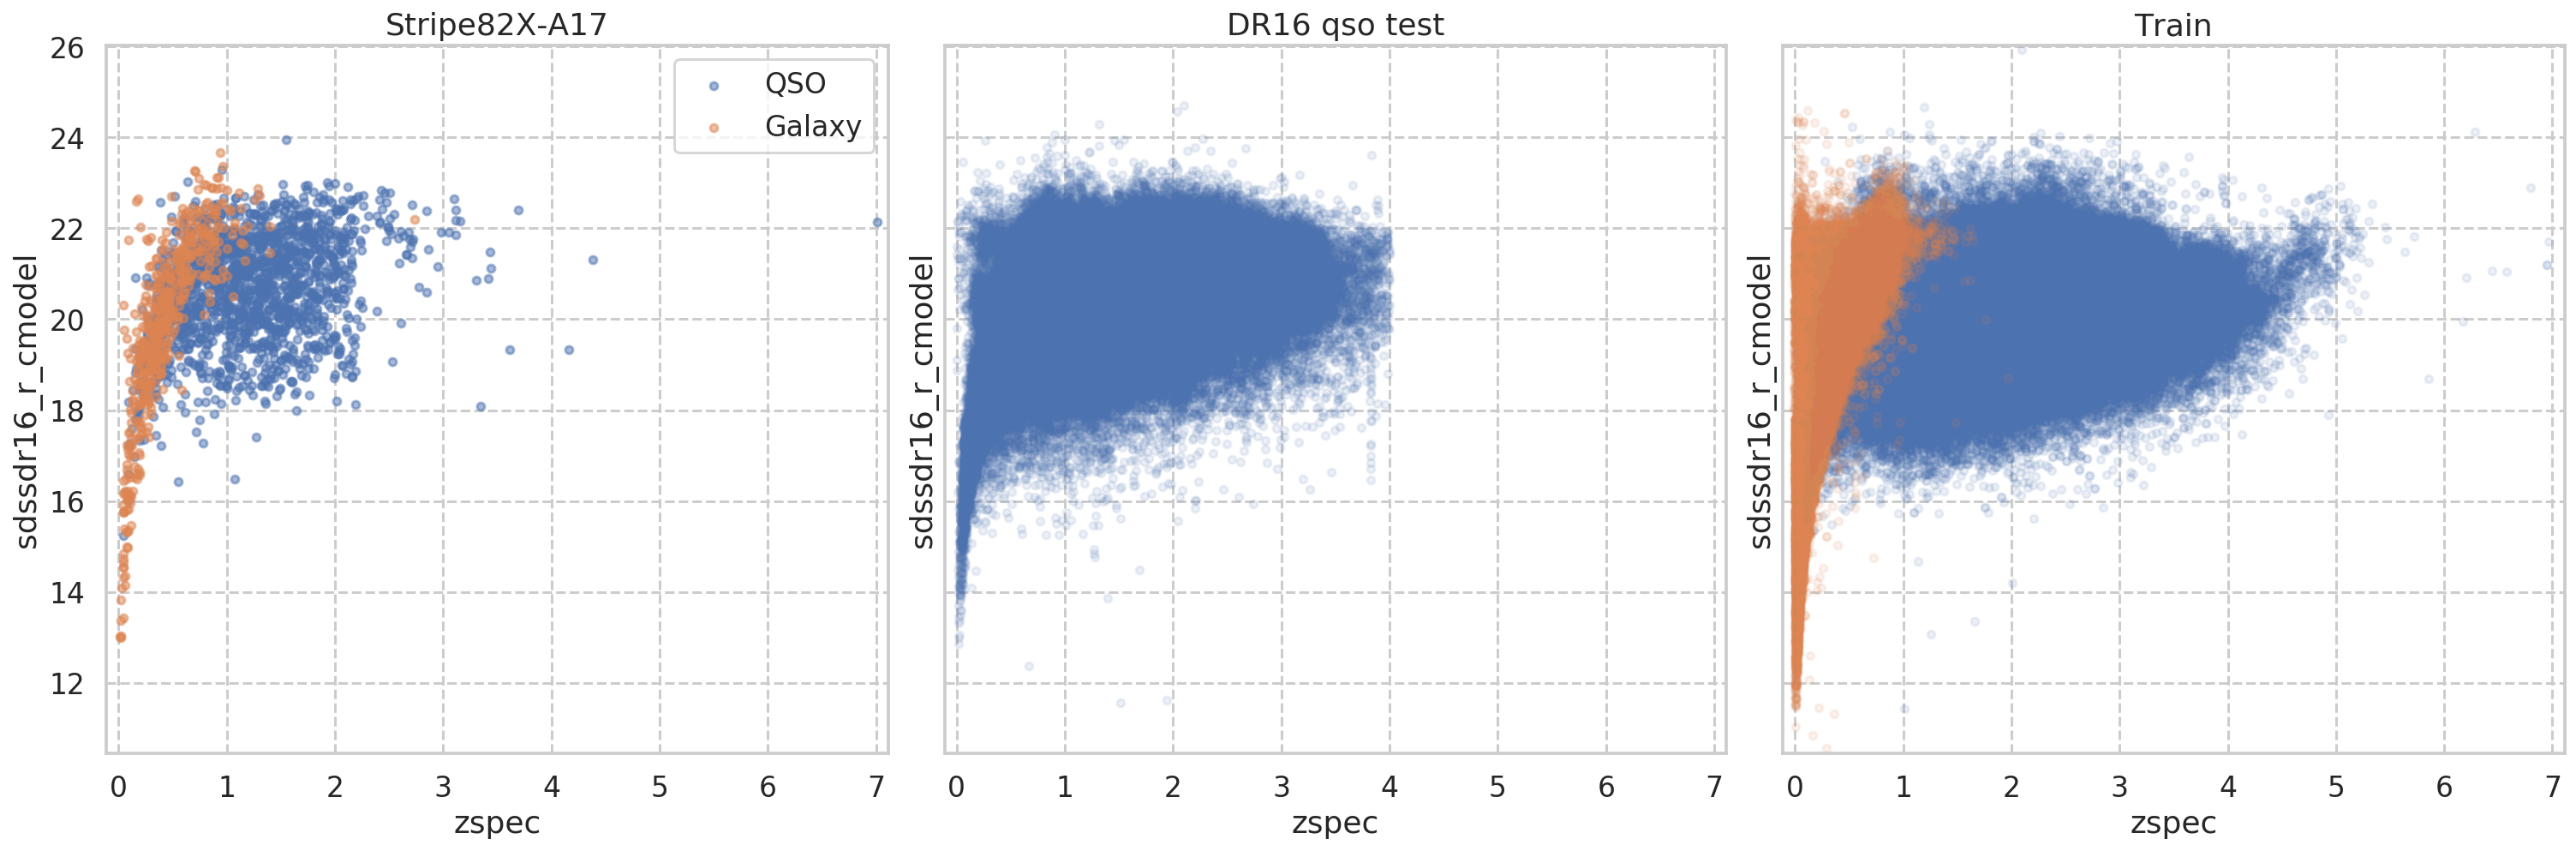
\includegraphics[width=\linewidth]{images/spectroscopic-coverage.png}
    \caption{Spectroscopic coverage of samples}
    \label{fig:spectroscopic_coverage}
\end{figure*}

\subsubsection{SDSS}

Описание числа объектов спектраальной выборки SDSS.

Сказать про DR14q Paris, и как отбираются надежные объекты DR16. Привести картинку из презенташки.

\subsubsection{Stripe82X}

Не уверен, где лучше описать выборку - тут или в \ref{sebsebsec:test}?

Вкратце описать выборку, что она из себя представляет, что это наилучший тест для рентгеновских квазаров, сослаться на работу Ananna.

\subsection{Datasets}

\subsubsection{Train}

Как составлены обучающие выборки (рентгеновская, оптическая).

Привести скаттерплоты zspec(mag\_r), как в Brescia, чтобы показать спектроскопическое покрытие ("spectroscopic coverage"), сравнить его со Stripe82X

\subsubsection{Test}\label{sebsebsec:test}

Описание выборки 200 тыс. квазаров, как составлена. Что мы её используем, чтобы, в первую очередь, адекватно протестироваться на далеких объектах.

+ В качестве теста используем Stripe82X.

+ для обеих выборок привести спектроскопическое покрытие.
\section{Models}\label{sec:algos}

\subsection{Feature Extraction}

Идея: нет идеального алгоритма Feature Importance, поэтому фичи выбираем экспертно из общих соображений. Но это надо обосновать.

Описать логику выбора признаков.

\achtung{тут же про ebv}

\subsection{Random Forests}
Описание случайного леса. Выбор случайного леса - сослаться на статью LSST.

\subsection{Adoptation of Random Forest for probabilistic photo-z predictions}
Описание, как адаптировали случайный лес.

\subsubsection{KDE}
Как определять ширину ядра. Как потом сравнивать прогнозы?

\subsubsection{Domain Adoptation}
Обучающая выборка - спектральная выборка оптических, а целевая - фотометрическая рентгеновских объектов.

\subsubsection{Photometric errors perturbations}

Как разыгрываем ошибки.

\subsection{Classification of stars}
Описание алгоритма классификации.
\section{Metrics}

To evaluate photo-z point estimates accuracy we use metrics common for this area [Salvato, Brescia, etc.]:
\begin{itemize}

    % \item root mean square error
    % \begin{equation}\label{eq:rmse}
    %     RMSE = \sqrt{\frac{1}{N} \sum_{i=1}^{N}\delta z_i ^2}
    % \end{equation}
    
    \item normalized median absolute deviation
    \begin{equation}\label{eq:nmad}
        NMAD = 1.4826 \times median(|\delta z_i|)
    \end{equation}{}
    
    \item fraction of catastrophic outliers
    \begin{equation}\label{eq:catout_formula}
        n_{>0.15} = \frac{N_{\delta z_i > 0.15}}{N}; N_{\delta z_i > 0.15} = \#\{i | \delta z_i > 0.15\},
    \end{equation}{}
    
    % \item bias
    % \begin{equation}
    %     \mu = \frac{1}{N_{\delta z_i \leq 0.15}} \sum_{i|\delta z_i \leq 0.15} \delta z_i
    % \end{equation}
    
    \item where \(\delta z_i\) defined as
    \begin{equation}\label{eq:deltaznorm}
    \delta z_i = \frac{\Delta z_i}{1+z_{spec,i}} = \frac{z_{ph,i} - z_{spec,i}}{1+z_{spec,i}}
\end{equation}
    
\end{itemize}        
\section{Results}\label{sec:exps}

\subsection{Models based on various features}

Описание экспериментов по построению моделей. Основная цель эксперимента - улучшение качества моделей за счет использования более глубоких данных. Базовая модель - SDSS. + описать сравнение моделей на, обученных на рентгеновской выборке vs обученных на оптической.

\subsection{Models based on various trains}

\subsection{Photometric errors}

Здесь про разыгрывание ошибок. Сначала описание 22ой модели, что у неё не скоррелированы признаки, поэтому можно спокойно разыгрывать ошибки (м.б. посчитать корелляцию Пирсона для всех признаков?), потом сравнение до-после по точности.

\subsection{ebv}

Примерно так же, но про поглощение.

\subsection{Best models detailed comparison}

\achtung{Эта часть самая важная. Её нужно продумать.}

\achtung{Сделать таблицы и графики, которые здесь хочется видеть. Тезисно изложить эту часть вместе с картинками}

\achtung{Тут рассказать про отдельно далекие/близкие, яркие/слабые, для 15!, (17?), 19!, (21?!), 22, 35!}

\subsubsection{Photo-z accuracy}

В таблице \ref{tab:metrics-s82x-a17-all30sec} приведены метрики... Видно, что лучшая из предложенных моделей превосходит модели SOTA в 2 раза по метрикам.

Сравнение на точечных и протяженных источниках.

Точность photo-z по метрикам NMAD, catout (каким еще?) на выборке 200 тыс. квазаров моделей 15, 17, 19, 21, 22, 35. Сравнение с Ananna, Brescia на Stripe82X.


Как лучше показывать метрики в бинах? Как в \ref{tab:metrics-by-rmag-s82x-a17} или графики, которые я построил недавно. 

Где-нибудь привести примеры спектров и прогнозов из "красной подложки". Думаю, это будет очень интересно. Описание паттернов ошибок? Тогда нужно добавить скаттерплоты на выборке квазаров.

Описать, что доля выбросов сильно растет на объектах с низким сигнал-шумом. При росте отношения сигнала к шуму точность растет.

Стоит описывать, что модели ведут себя неустойчиво в зависимости от spec-z?

\begin{figure*}
    \centering
    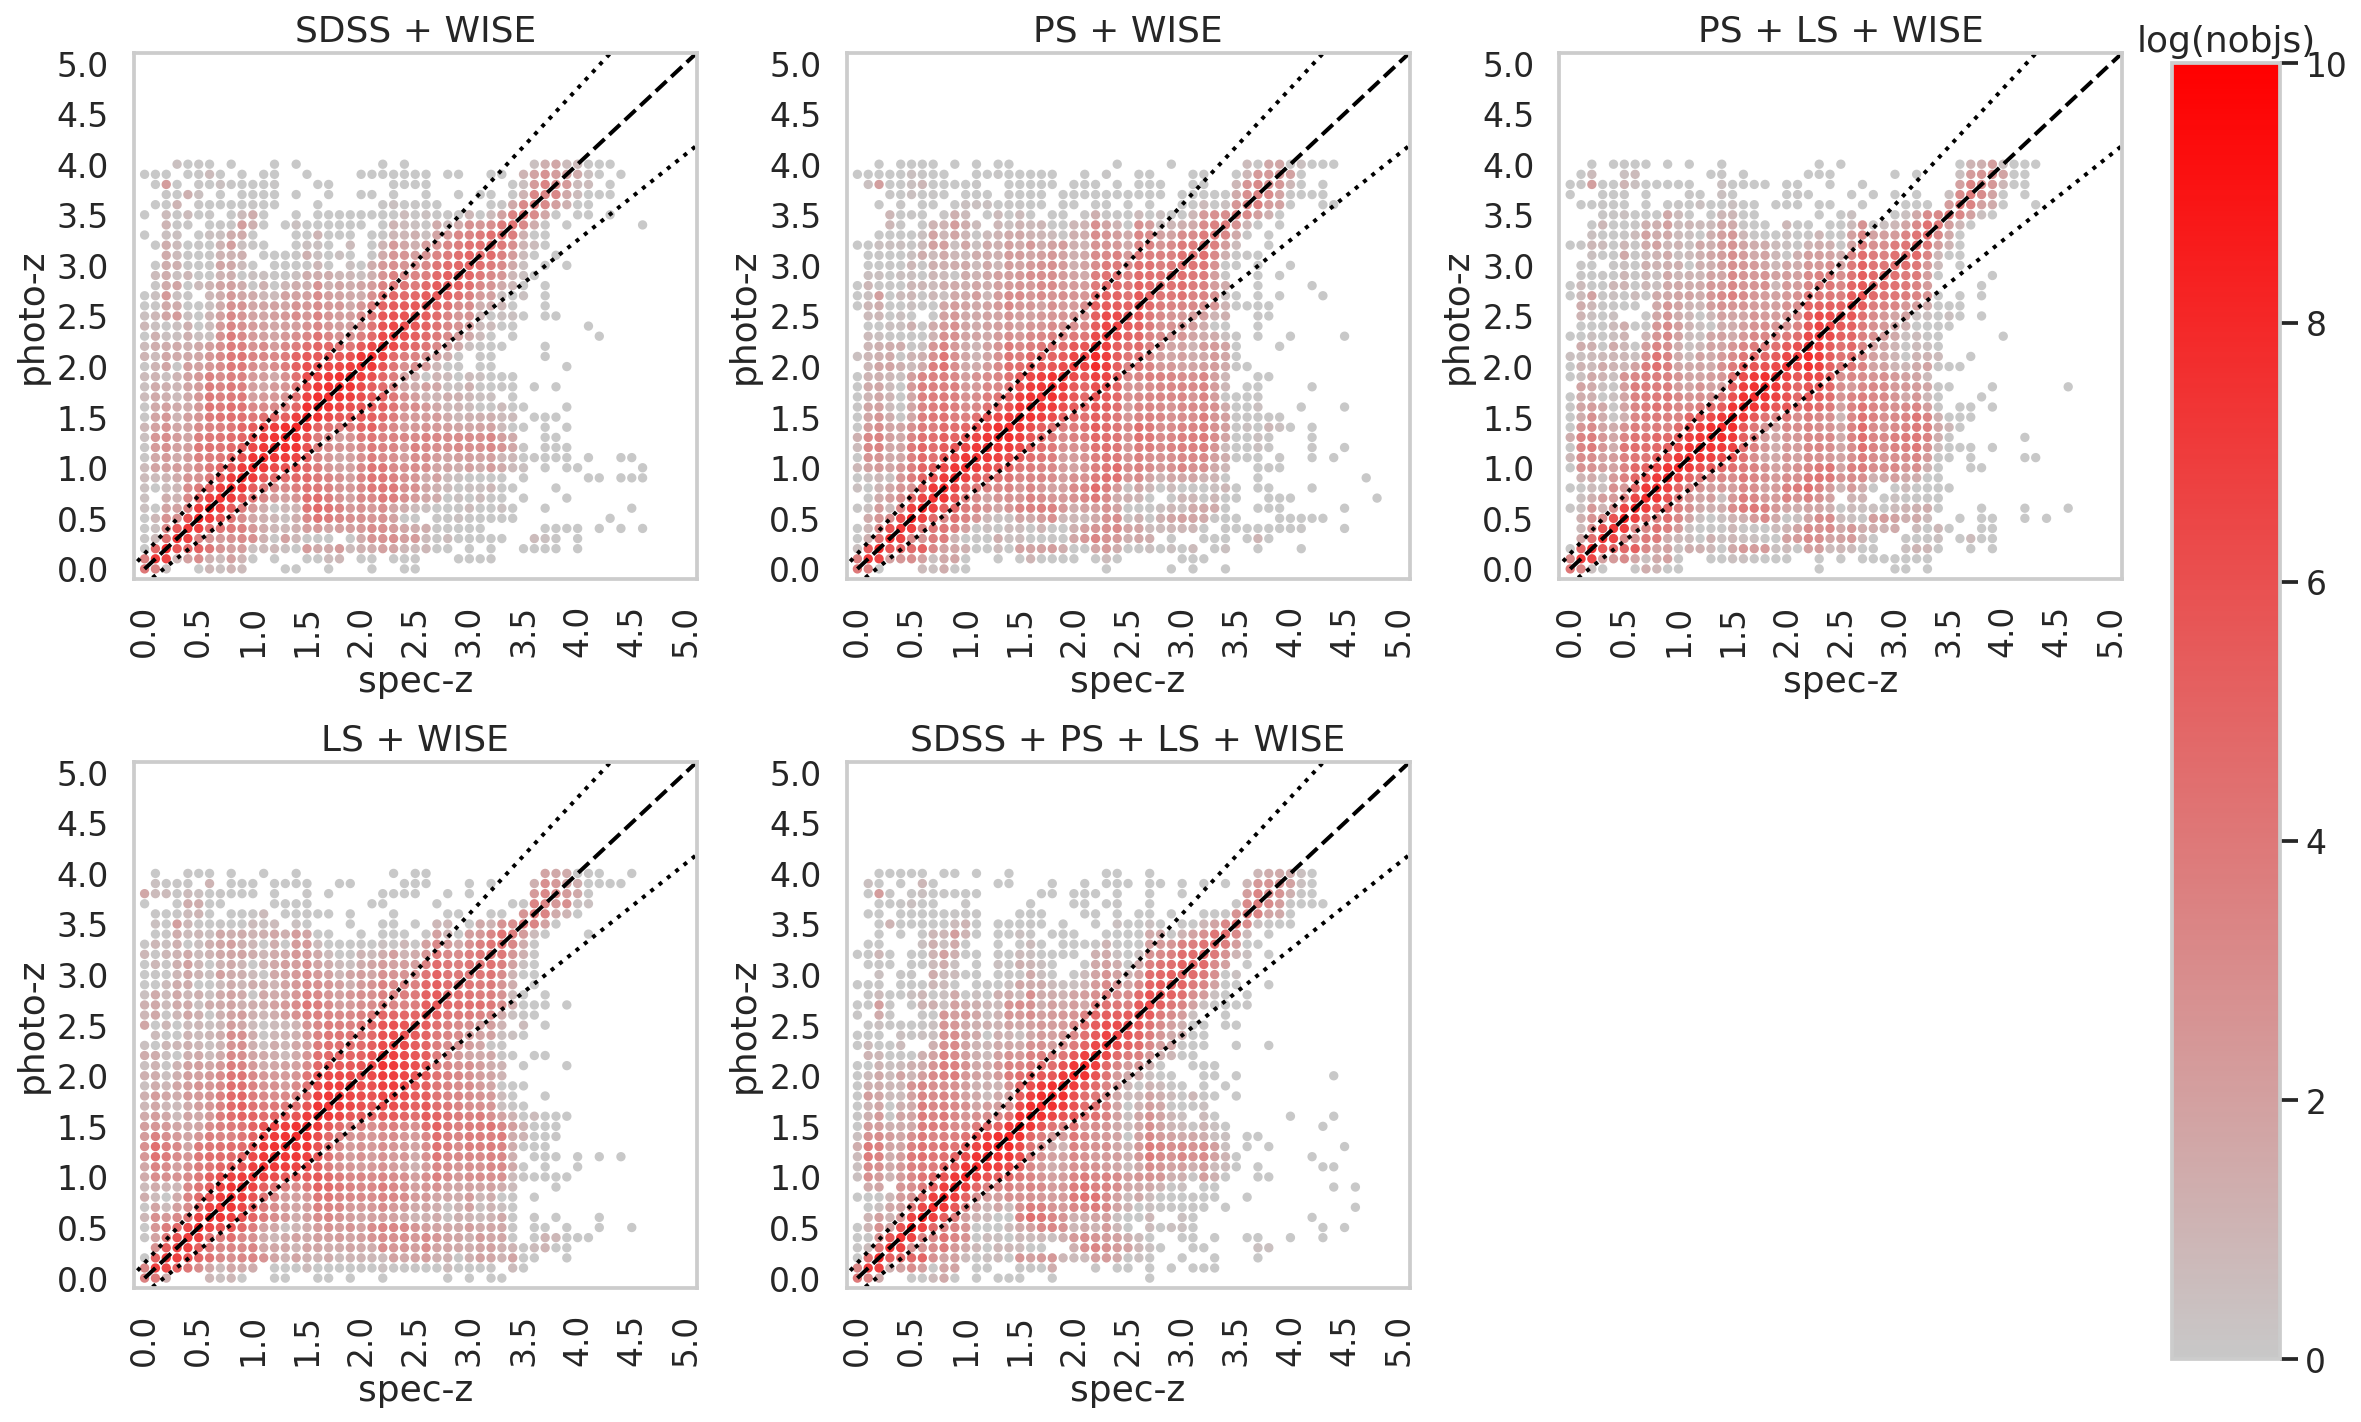
\includegraphics[width=\linewidth]{images/scatterplots-dr16qso.png}
    \caption{Scatterplots of catastrophic outliers on DR16 QSOs}
    \label{fig:my_label}
\end{figure*}

\begin{figure*}
    \centering
    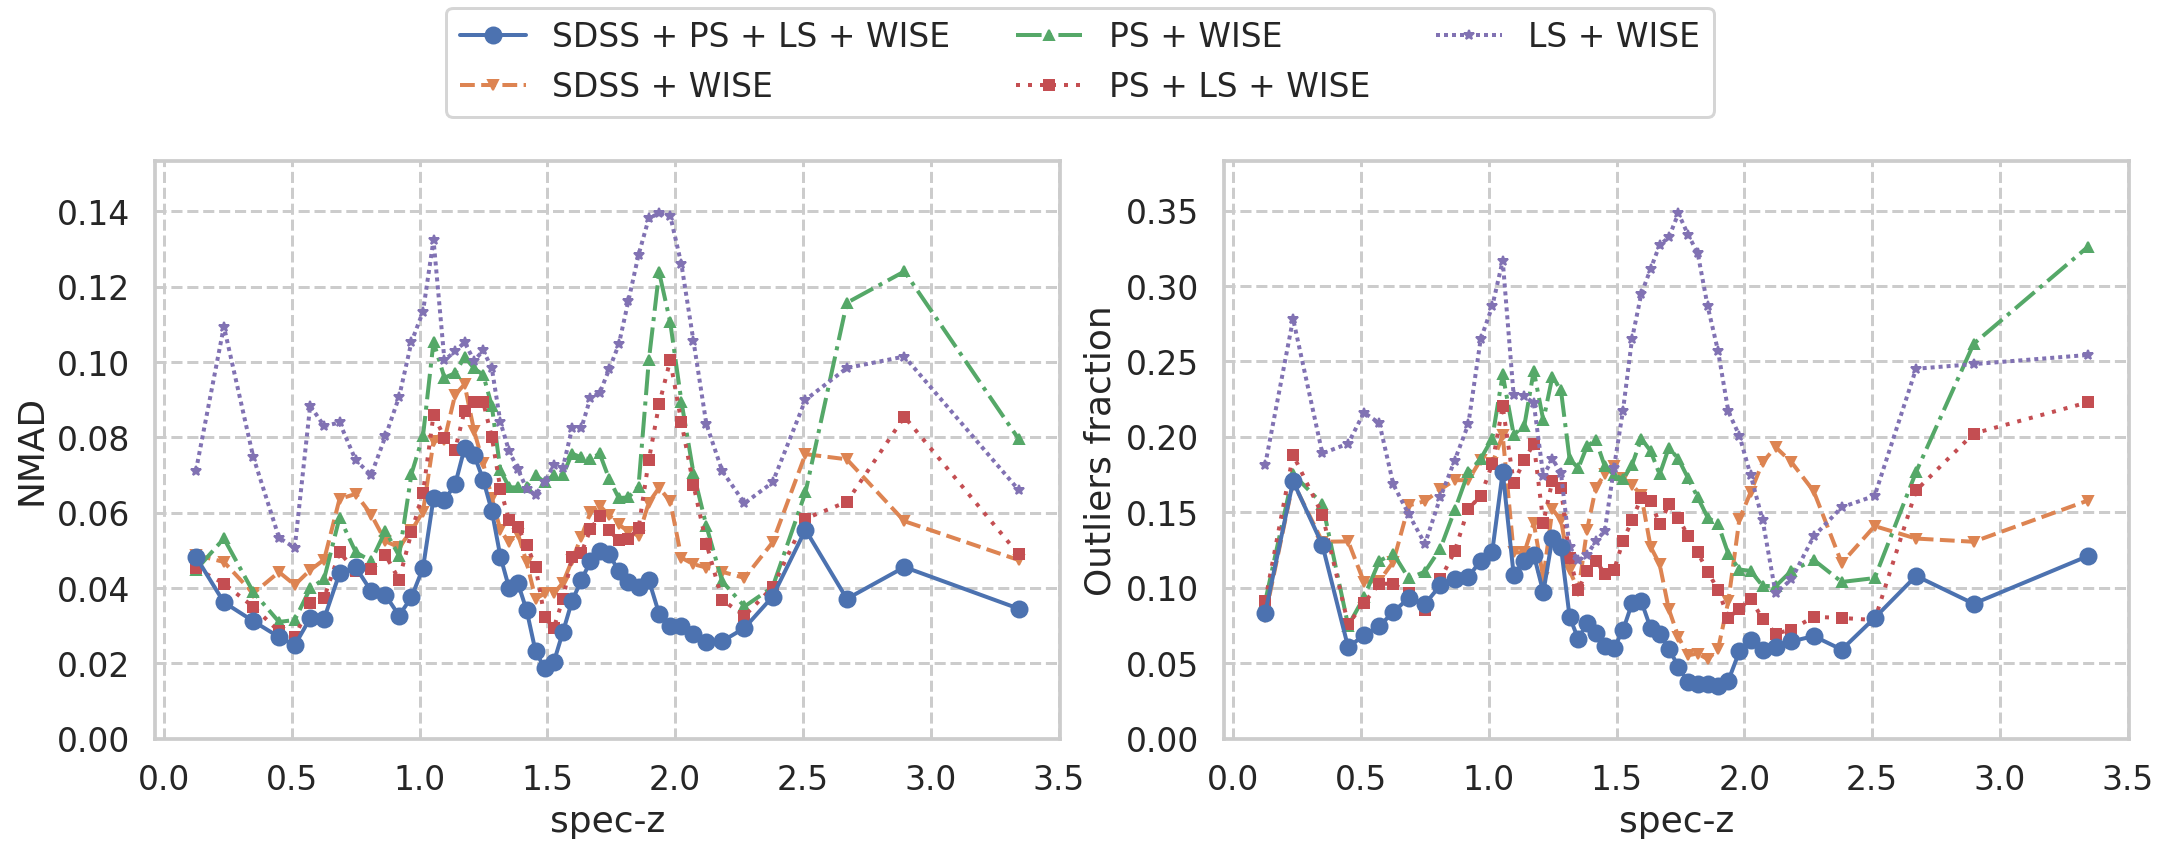
\includegraphics[width=\linewidth]{images/metrics-dr16qso-zspec.png}
    \caption{Метрики на квазарах DR16}
    \label{fig:my_label}
\end{figure*}

\begin{figure*}
    \centering
    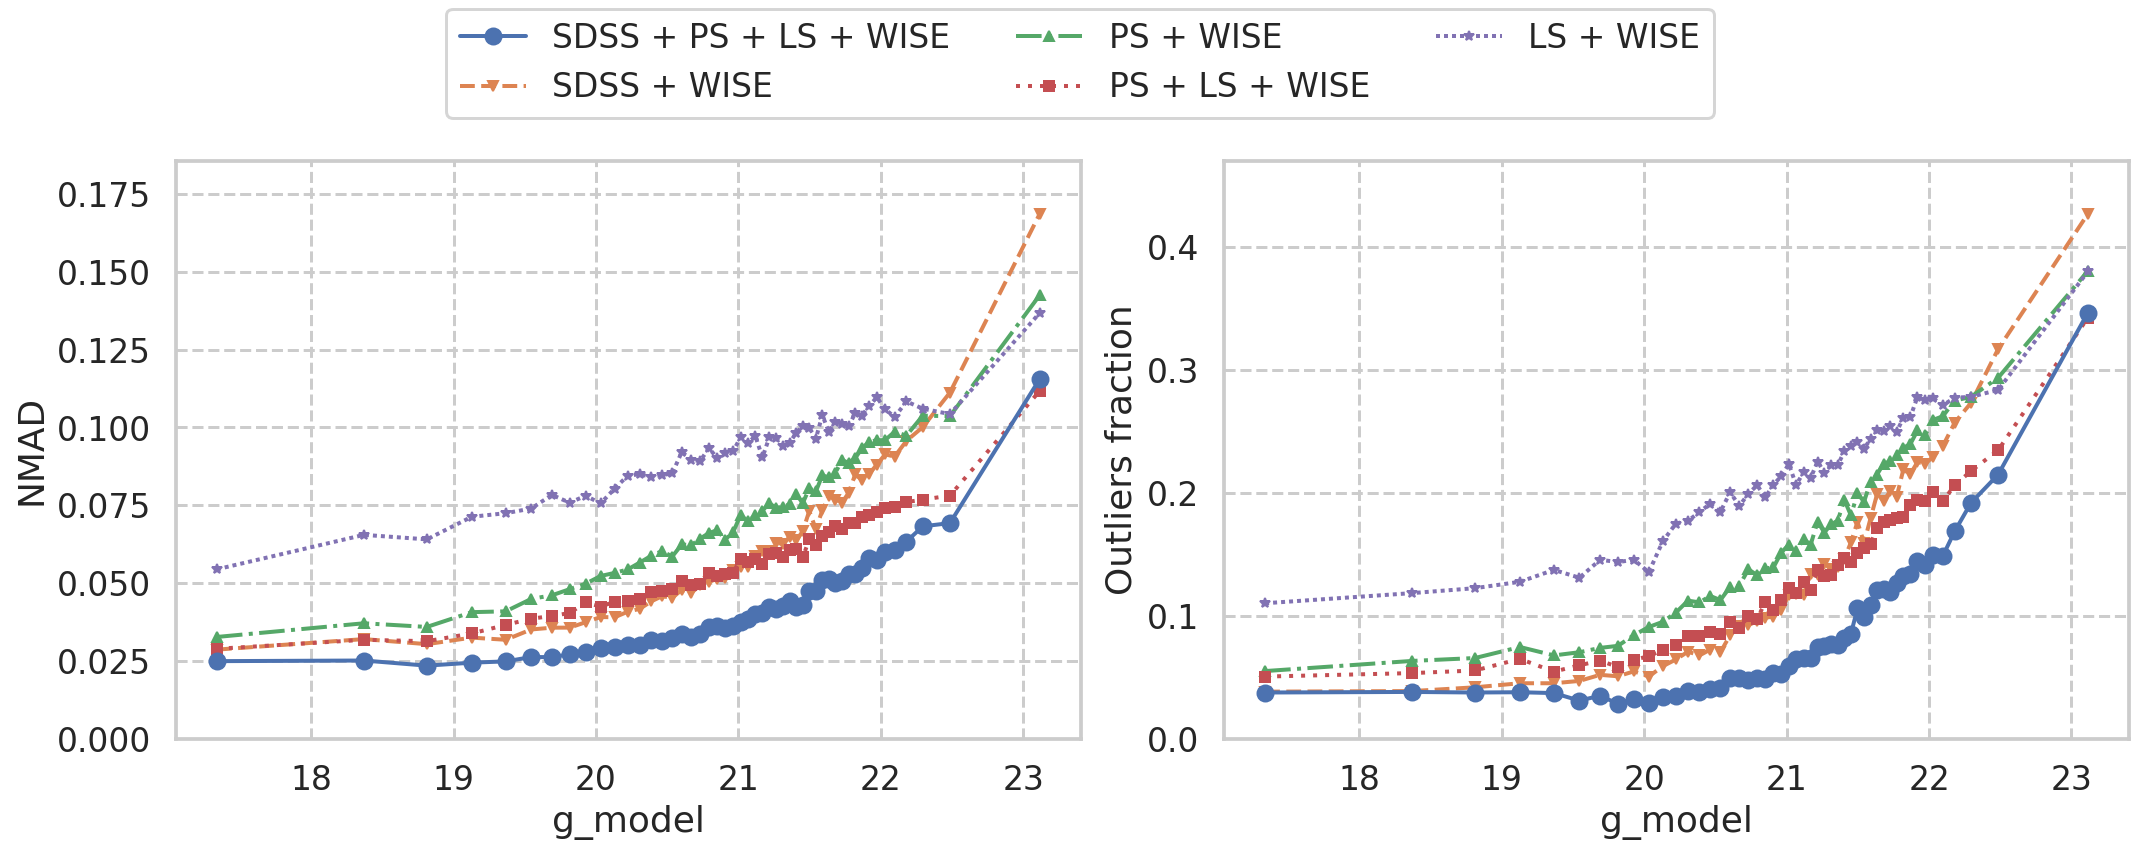
\includegraphics[width=\linewidth]{images/metrics-dr16qso-gmag.png}
    \caption{Метрики на квазарах DR16}
    \label{fig:metrics-dr16qso-gmag}
\end{figure*}

\begin{figure*}
    \centering
    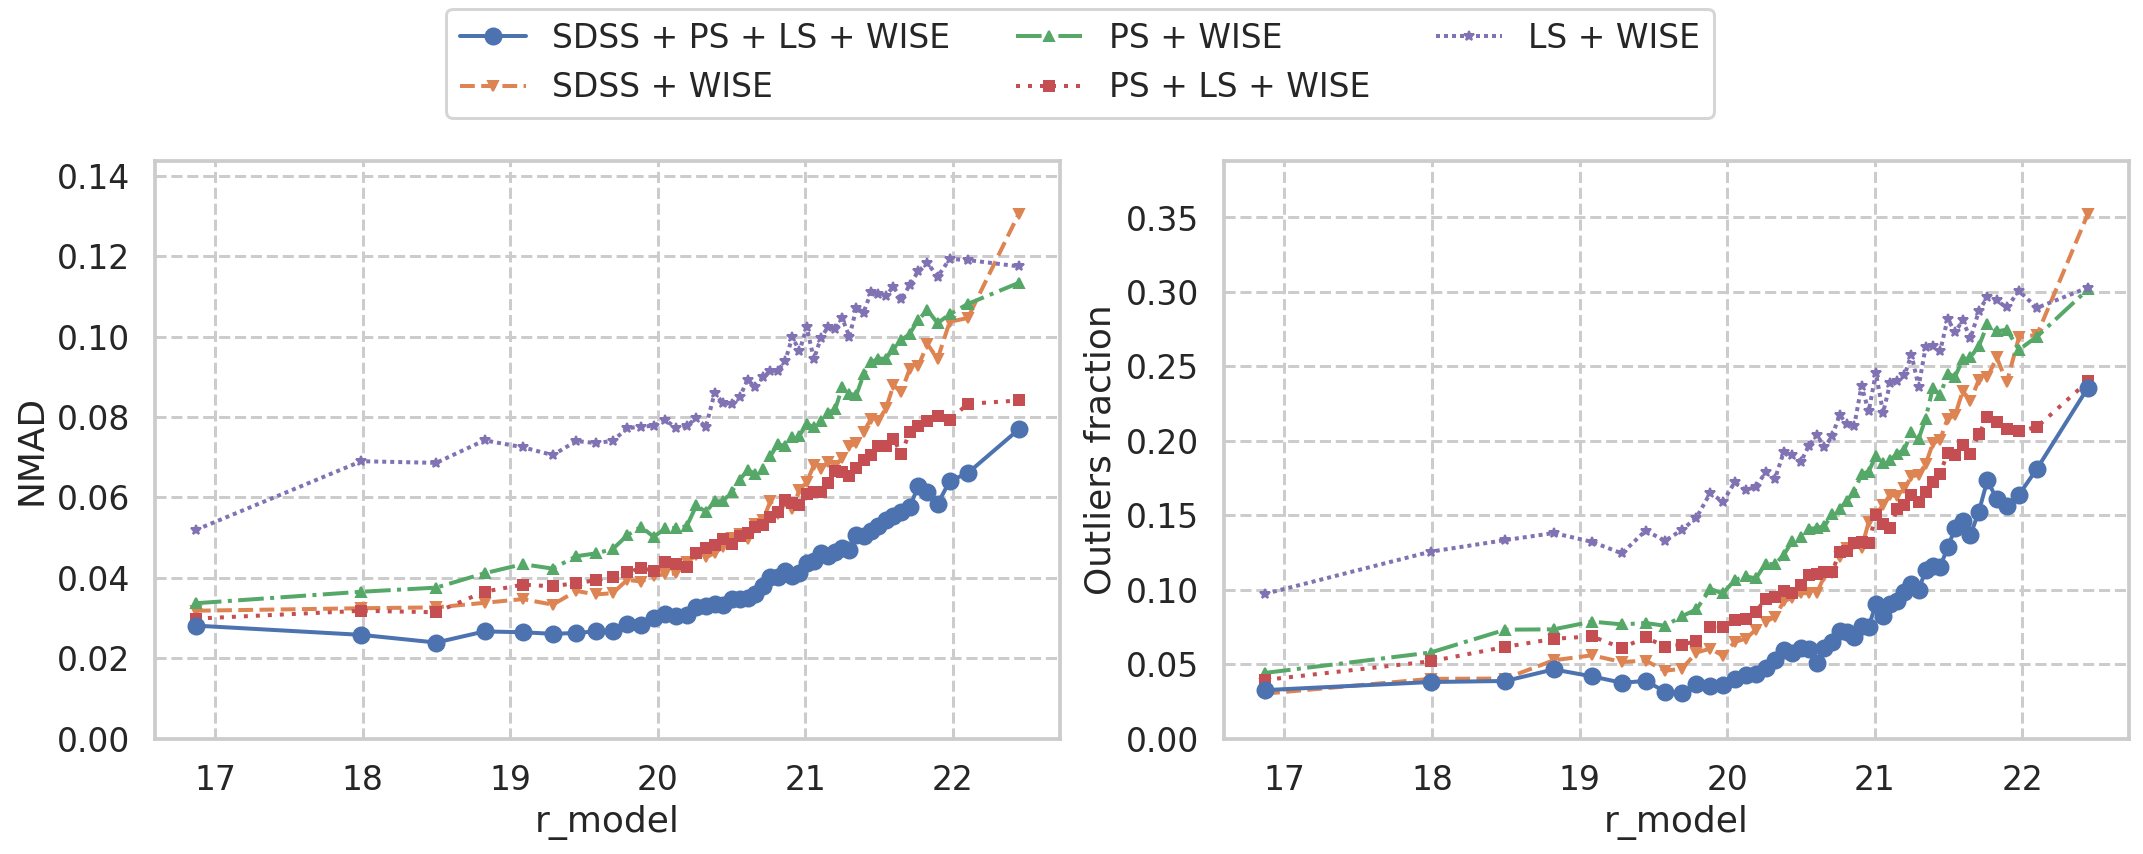
\includegraphics[width=\linewidth]{images/metrics-dr16qso-rmag.png}
    \caption{Метрики на квазарах DR16}
    \label{fig:metrics-dr16qso-sng}
\end{figure*}

\begin{figure*}
    \centering
    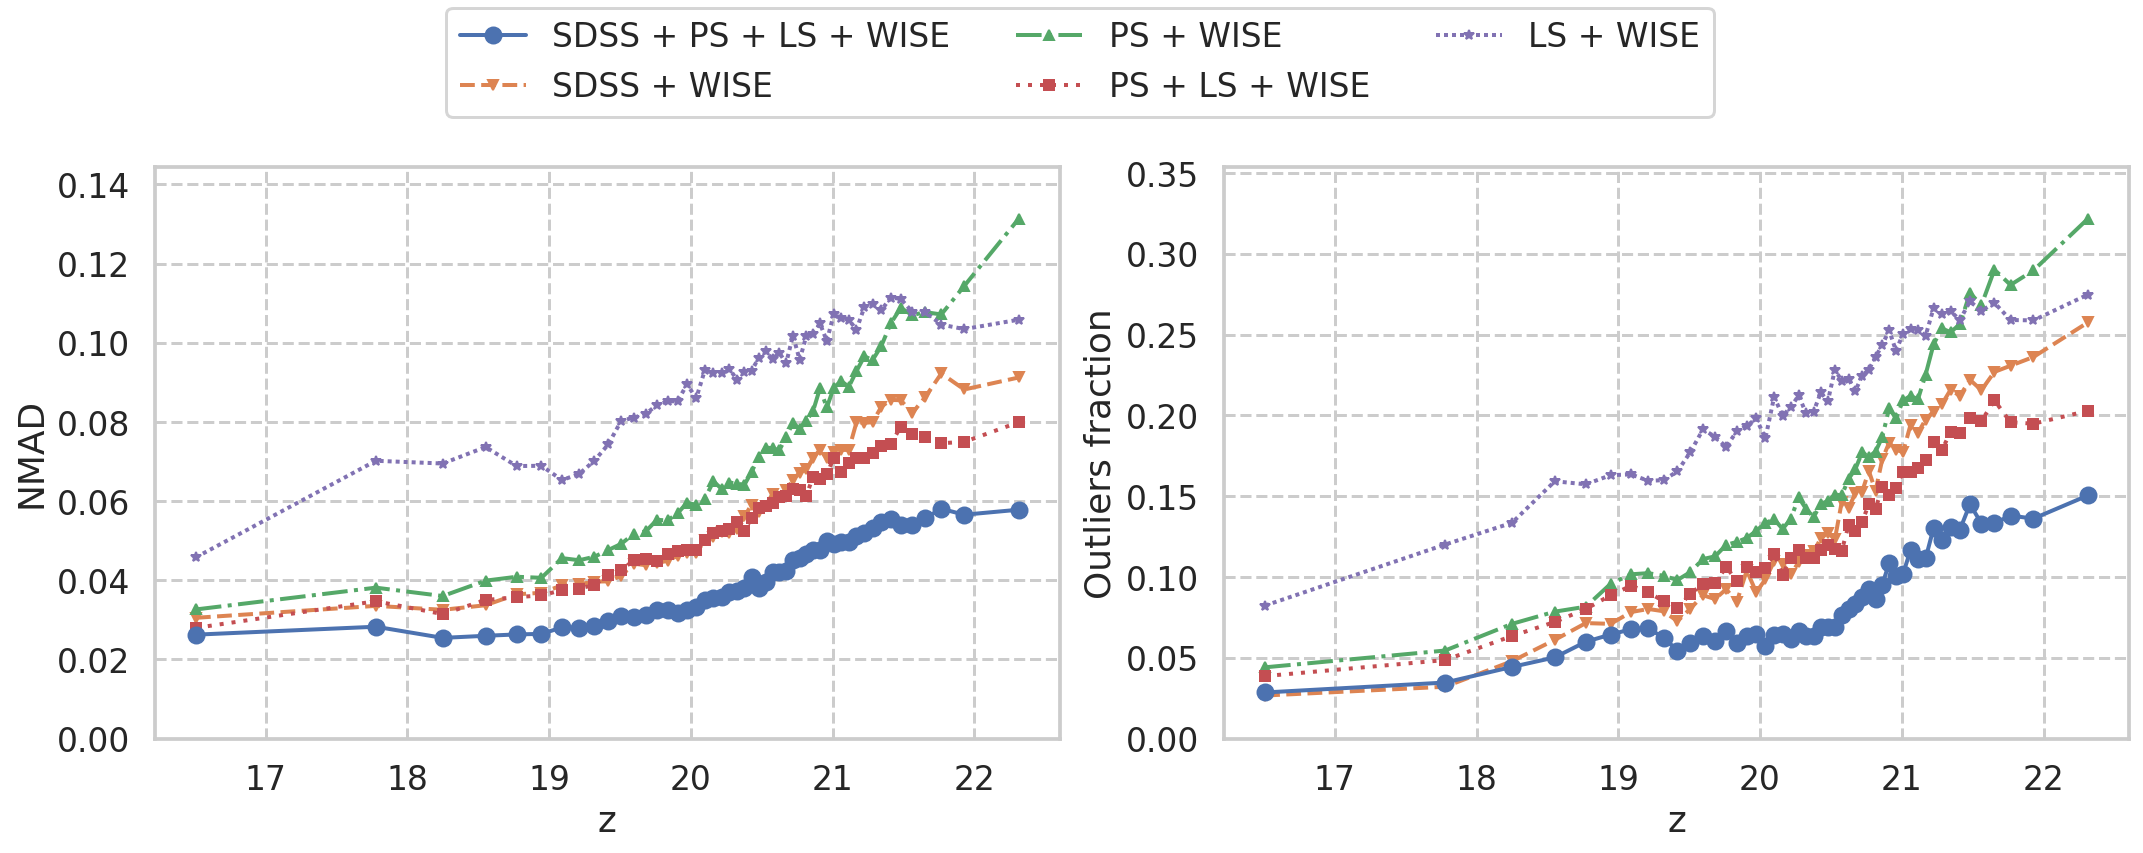
\includegraphics[width=\linewidth]{images/metrics-dr16qso-zmag.png}
    \caption{Метрики на квазарах DR16}
    \label{fig:metrics-dr16qso-snw1}
\end{figure*}

\begin{figure*}
    \centering
    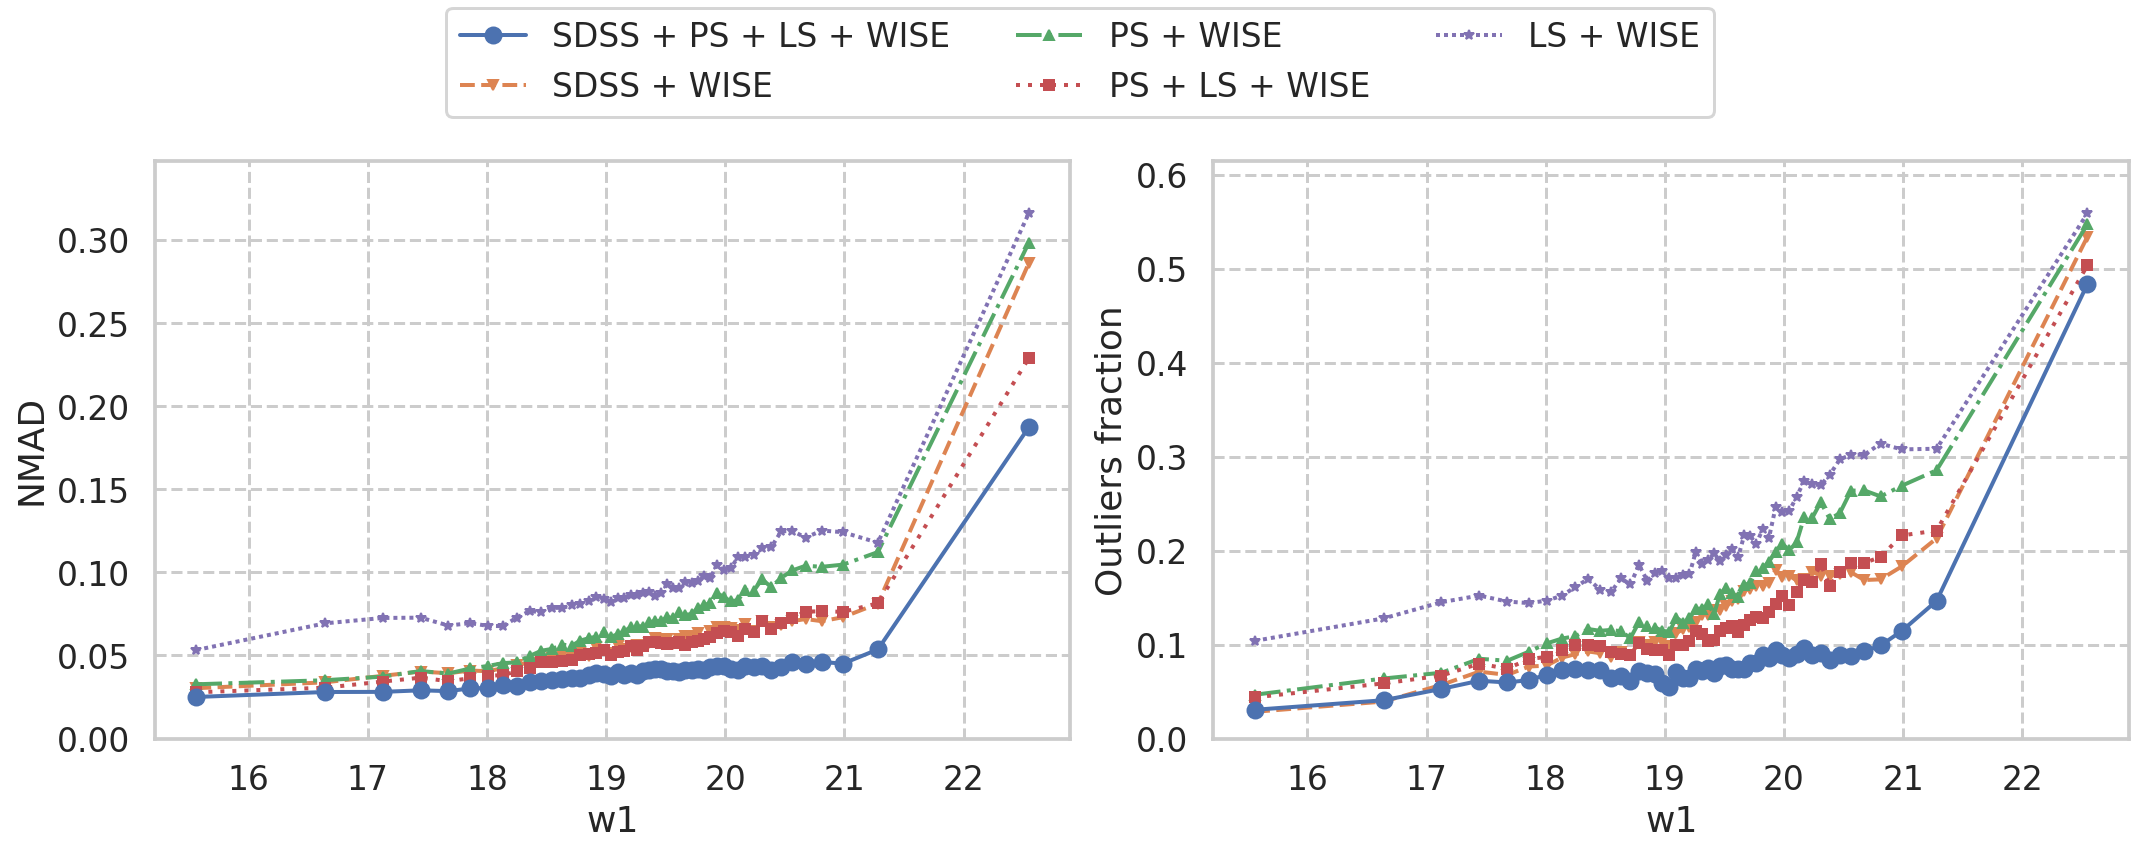
\includegraphics[width=\linewidth]{images/metrics-dr16qso-w1mag.png}
    \caption{Метрики на квазарах DR16}
    \label{fig:metrics-dr16qso-w1mag}
\end{figure*}

\begin{table*}
    \centering
    \begin{tabular}{lll}
    \hline
                        Model &   Dataset &                      All Objects \\
    \hline
                  SDSS + WISE &  S82X-A17 &                    0.049 / 0.127 \\
                  SDSS + WISE &  DR16 QSO &                    0.056 / 0.136 \\
                    PS + WISE &  S82X-A17 &                    0.059 / 0.153 \\
                    PS + WISE &  DR16 QSO &                    0.067 / 0.165 \\
                    LS + WISE &  S82X-A17 &                    0.076 / 0.177 \\
                    LS + WISE &  DR16 QSO &                    0.090 / 0.212 \\
        SDSS + PS + LS + WISE &  S82X-A17 &  \textbf{0.034} / \textbf{0.080} \\
        SDSS + PS + LS + WISE &  DR16 QSO &  \textbf{0.039} / \textbf{0.084} \\
     Templates (Ananna, 2017) &  S82X-A17 &                    0.065 / 0.170 \\
          ANN (Brescia, 2019) &  S82X-A17 &                    0.066 / 0.156 \\
                        nobjs &  S82X-A17 &                             2664 \\
                        nobjs &  DR16 QSO &                           211903 \\
    \hline
    \end{tabular}
    
    \caption{Метрики предложенных моделей и SOTA на тестовых выборках}
    \label{tab:metrics-rmag}
\end{table*}


\begin{table*}
    \centering
    \begin{tabular}{lllllll}
    \hline
                        Model &   Dataset &                         r < 19.5 &                  19.5 < r < 20.5 &                    20.5 < r < 21 &                    21 < r < 21.5 &                    21.5 < r < 23 \\
    \hline
                  SDSS + WISE &  S82X-A17 &                    0.028 / 0.031 &                    0.040 / 0.045 &                    0.058 / 0.115 &                    0.069 / 0.191 &                    0.098 / 0.285 \\
                  SDSS + WISE &  DR16 QSO &                    0.033 / 0.046 &                    0.042 / 0.069 &                    0.056 / 0.119 &                    0.071 / 0.177 &                    0.095 / 0.252 \\
                    PS + WISE &  S82X-A17 &                    0.031 / 0.046 &                    0.049 / 0.083 &                    0.063 / 0.138 &                    0.086 / 0.210 &                    0.107 / 0.313 \\
                    PS + WISE &  DR16 QSO &                    0.040 / 0.069 &                    0.053 / 0.105 &                    0.069 / 0.157 &                    0.085 / 0.206 &                    0.103 / 0.267 \\
                    LS + WISE &  S82X-A17 &                    0.050 / 0.069 &                    0.076 / 0.150 &                    0.078 / 0.182 &                    0.082 / 0.184 &                    0.109 / 0.303 \\
                    LS + WISE &  DR16 QSO &                    0.068 / 0.127 &                    0.079 / 0.166 &                    0.091 / 0.211 &                    0.103 / 0.249 &                    0.115 / 0.288 \\
        SDSS + PS + LS + WISE &  S82X-A17 &  \textbf{0.023} / \textbf{0.027} &  \textbf{0.028} / \textbf{0.031} &  \textbf{0.038} / \textbf{0.057} &  \textbf{0.044} / \textbf{0.116} &  \textbf{0.064} / \textbf{0.181} \\
        SDSS + PS + LS + WISE &  DR16 QSO &  \textbf{0.026} / \textbf{0.039} &  \textbf{0.030} / \textbf{0.043} &  \textbf{0.038} / \textbf{0.067} &  \textbf{0.048} / \textbf{0.102} &  \textbf{0.060} / \textbf{0.163} \\
     Templates (Ananna, 2017) &  S82X-A17 &                    0.061 / 0.099 &                    0.061 / 0.137 &                    0.061 / 0.170 &                    0.069 / 0.219 &                    0.082 / 0.247 \\
          ANN (Brescia, 2019) &  S82X-A17 &                    0.062 / 0.102 &                    0.057 / 0.125 &                    0.060 / 0.140 &                    0.073 / 0.209 &                    0.084 / 0.222 \\
                        nobjs &  S82X-A17 &                              586 &                              686 &                              407 &                              398 &                              576 \\
                        nobjs &  DR16 QSO &                            29085 &                            53555 &                            41596 &                            43574 &                            43934 \\
    \hline
    \end{tabular}
    
    \caption{Метрики предложенных моделей и SOTA на тестовых выборках в бинах по r}
    \label{tab:metrics-rmag}
\end{table*}


\begin{table*}
    \centering
    \begin{tabular}{lllllll}
    \hline
                        Model &   Dataset &                           g < 20 &                      20 < g < 21 &                    21 < g < 21.5 &                    21.5 < g < 22 &                      22 < g < 24 \\
    \hline
                  SDSS + WISE &  S82X-A17 &                    0.027 / 0.028 &                    0.042 / 0.062 &                    0.061 / 0.122 &                    0.063 / 0.170 &                    0.108 / 0.299 \\
                  SDSS + WISE &  DR16 QSO &                    0.033 / 0.046 &                    0.046 / 0.081 &                    0.062 / 0.137 &                    0.078 / 0.200 &                    0.104 / 0.289 \\
                    PS + WISE &  S82X-A17 &                    0.032 / 0.046 &                    0.050 / 0.110 &                    0.060 / 0.144 &                    0.082 / 0.221 &                    0.099 / 0.295 \\
                    PS + WISE &  DR16 QSO &                    0.042 / 0.070 &                    0.061 / 0.122 &                    0.074 / 0.172 &                    0.088 / 0.226 &                    0.104 / 0.290 \\
                    LS + WISE &  S82X-A17 &                    0.054 / 0.083 &                    0.078 / 0.173 &                    0.078 / 0.183 &                    0.083 / 0.171 &                    0.099 / 0.285 \\
                    LS + WISE &  DR16 QSO &                    0.070 / 0.131 &                    0.087 / 0.188 &                    0.096 / 0.223 &                    0.102 / 0.255 &                    0.109 / 0.293 \\
        SDSS + PS + LS + WISE &  S82X-A17 &  \textbf{0.021} / \textbf{0.020} &  \textbf{0.030} / \textbf{0.046} &  \textbf{0.035} / \textbf{0.058} &  \textbf{0.043} / \textbf{0.095} &  \textbf{0.073} / \textbf{0.198} \\
        SDSS + PS + LS + WISE &  DR16 QSO &  \textbf{0.026} / \textbf{0.035} &  \textbf{0.033} / \textbf{0.044} &  \textbf{0.042} / \textbf{0.075} &  \textbf{0.053} / \textbf{0.124} &  \textbf{0.068} / \textbf{0.201} \\
     Templates (Ananna, 2017) &  S82X-A17 &                    0.061 / 0.110 &                    0.058 / 0.135 &                    0.068 / 0.192 &                    0.071 / 0.206 &                    0.085 / 0.246 \\
          ANN (Brescia, 2019) &  S82X-A17 &                    0.062 / 0.115 &                    0.055 / 0.119 &                    0.069 / 0.159 &                    0.075 / 0.187 &                    0.083 / 0.231 \\
                        nobjs &  S82X-A17 &                              609 &                              725 &                              433 &                              359 &                              529 \\
                        nobjs &  DR16 QSO &                            38951 &                            59379 &                            43883 &                            44277 &                            25123 \\
    \hline
    \end{tabular}
    
    \caption{Метрики предложенных моделей и SOTA на тестовых выборках в бинах по g}
    \label{tab:metrics-rmag}
\end{table*}


\begin{table*}
    \centering
    \begin{tabular}{lllllll}
    \hline
                        Model &   Dataset &                           z < 19 &                      19 < z < 20 &                    20 < z < 20.5 &                    20.5 < z < 21 &                      21 < z < 23 \\
    \hline
                  SDSS + WISE &  S82X-A17 &                    0.030 / 0.029 &                    0.040 / 0.060 &                    0.050 / 0.098 &                    0.065 / 0.176 &                    0.099 / 0.284 \\
                  SDSS + WISE &  DR16 QSO &                    0.034 / 0.051 &                    0.042 / 0.085 &                    0.053 / 0.112 &                    0.066 / 0.157 &                    0.082 / 0.214 \\
                    PS + WISE &  S82X-A17 &                    0.031 / 0.044 &                    0.046 / 0.077 &                    0.063 / 0.123 &                    0.079 / 0.199 &                    0.119 / 0.335 \\
                    PS + WISE &  DR16 QSO &                    0.038 / 0.070 &                    0.051 / 0.111 &                    0.064 / 0.139 &                    0.079 / 0.176 &                    0.102 / 0.257 \\
                    LS + WISE &  S82X-A17 &                    0.046 / 0.067 &                    0.075 / 0.134 &                    0.077 / 0.187 &                    0.084 / 0.199 &                    0.109 / 0.305 \\
                    LS + WISE &  DR16 QSO &                    0.065 / 0.135 &                    0.078 / 0.179 &                    0.092 / 0.205 &                    0.099 / 0.232 &                    0.107 / 0.261 \\
        SDSS + PS + LS + WISE &  S82X-A17 &  \textbf{0.023} / \textbf{0.027} &  \textbf{0.028} / \textbf{0.036} &  \textbf{0.035} / \textbf{0.071} &  \textbf{0.040} / \textbf{0.086} &  \textbf{0.060} / \textbf{0.182} \\
        SDSS + PS + LS + WISE &  DR16 QSO &  \textbf{0.026} / \textbf{0.047} &  \textbf{0.030} / \textbf{0.063} &  \textbf{0.037} / \textbf{0.064} &  \textbf{0.045} / \textbf{0.088} &  \textbf{0.054} / \textbf{0.129} \\
     Templates (Ananna, 2017) &  S82X-A17 &                    0.063 / 0.091 &                    0.062 / 0.146 &                    0.058 / 0.145 &                    0.061 / 0.186 &                    0.085 / 0.279 \\
          ANN (Brescia, 2019) &  S82X-A17 &                    0.063 / 0.091 &                    0.059 / 0.137 &                    0.056 / 0.127 &                    0.063 / 0.159 &                    0.090 / 0.257 \\
                        nobjs &  S82X-A17 &                              552 &                              665 &                              440 &                              408 &                              587 \\
                        nobjs &  DR16 QSO &                            24762 &                            46885 &                            38244 &                            44079 &                            57843 \\
    \hline
    \end{tabular}
    
    \caption{Метрики предложенных моделей и SOTA на тестовых выборках в бинах по z}
    \label{tab:metrics-rmag}
\end{table*}


\begin{table*}
    \centering
    \begin{tabular}{lllllll}
    \hline
                        Model &   Dataset &                        w1 < 18.5 &                   18.5 < w1 < 19 &                   19 < w1 < 19.5 &                   19.5 < w1 < 20 &                   20 < w1 < 22.5 \\
    \hline
                  SDSS + WISE &  S82X-A17 &                    0.034 / 0.039 &                    0.047 / 0.093 &                    0.060 / 0.149 &                    0.067 / 0.201 &                    0.080 / 0.251 \\
                  SDSS + WISE &  DR16 QSO &                    0.040 / 0.071 &                    0.051 / 0.096 &                    0.056 / 0.123 &                    0.062 / 0.160 &                    0.072 / 0.189 \\
                    PS + WISE &  S82X-A17 &                    0.036 / 0.062 &                    0.054 / 0.080 &                    0.070 / 0.149 &                    0.093 / 0.223 &                    0.120 / 0.350 \\
                    PS + WISE &  DR16 QSO &                    0.042 / 0.090 &                    0.059 / 0.117 &                    0.067 / 0.133 &                    0.078 / 0.174 &                    0.098 / 0.254 \\
                    LS + WISE &  S82X-A17 &                    0.058 / 0.094 &                    0.070 / 0.130 &                    0.076 / 0.181 &                    0.093 / 0.226 &                    0.128 / 0.339 \\
                    LS + WISE &  DR16 QSO &                    0.069 / 0.146 &                    0.081 / 0.171 &                    0.086 / 0.184 &                    0.095 / 0.215 &                    0.118 / 0.293 \\
        SDSS + PS + LS + WISE &  S82X-A17 &  \textbf{0.026} / \textbf{0.031} &  \textbf{0.034} / \textbf{0.067} &  \textbf{0.039} / \textbf{0.079} &  \textbf{0.042} / \textbf{0.123} &  \textbf{0.046} / \textbf{0.150} \\
        SDSS + PS + LS + WISE &  DR16 QSO &  \textbf{0.030} / \textbf{0.061} &  \textbf{0.037} / \textbf{0.067} &  \textbf{0.040} / \textbf{0.069} &  \textbf{0.042} / \textbf{0.082} &  \textbf{0.045} / \textbf{0.109} \\
     Templates (Ananna, 2017) &  S82X-A17 &                    0.062 / 0.140 &                    0.072 / 0.161 &                    0.058 / 0.149 &                    0.072 / 0.216 &                    0.072 / 0.215 \\
          ANN (Brescia, 2019) &  S82X-A17 &                    0.062 / 0.136 &                    0.066 / 0.148 &                    0.056 / 0.117 &                    0.073 / 0.209 &                    0.083 / 0.195 \\
                        nobjs &  S82X-A17 &                              899 &                              460 &                              443 &                              393 &                              451 \\
                        nobjs &  DR16 QSO &                            46429 &                            29120 &                            39830 &                            40388 &                            54612 \\
    \hline
    \end{tabular}
    
    \caption{Метрики предложенных моделей и SOTA на тестовых выборках в бинах по w1}
    \label{tab:metrics-rmag}
\end{table*}


\begin{table*}
    \centering
    \begin{tabular}{lllllll}
    \hline
                        Model &   Dataset &             6e-15 < Fx < 9.8e-15 &           9.8e-15 < Fx < 1.5e-14 &           1.5e-14 < Fx < 2.5e-14 &             2.5e-14 < Fx < 4e-14 &                       4e-14 < Fx \\
    \hline
                  SDSS + WISE &  S82X-A17 &                    0.060 / 0.176 &                    0.048 / 0.123 &                    0.043 / 0.093 &                    0.040 / 0.064 &                    0.033 / 0.063 \\
                    PS + WISE &  S82X-A17 &                    0.069 / 0.180 &                    0.065 / 0.169 &                    0.054 / 0.129 &                    0.046 / 0.087 &                    0.034 / 0.085 \\
                    LS + WISE &  S82X-A17 &                    0.085 / 0.212 &                    0.074 / 0.183 &                    0.080 / 0.172 &                    0.069 / 0.144 &                    0.066 / 0.111 \\
        SDSS + PS + LS + WISE &  S82X-A17 &  \textbf{0.037} / \textbf{0.099} &  \textbf{0.034} / \textbf{0.073} &  \textbf{0.031} / \textbf{0.072} &  \textbf{0.028} / \textbf{0.042} &  \textbf{0.027} / \textbf{0.039} \\
     Templates (Ananna, 2017) &  S82X-A17 &                    0.061 / 0.164 &                    0.068 / 0.168 &                    0.066 / 0.184 &                    0.063 / 0.147 &                    0.074 / 0.219 \\
          ANN (Brescia, 2019) &  S82X-A17 &                    0.064 / 0.149 &                    0.070 / 0.162 &                    0.063 / 0.159 &                    0.065 / 0.125 &                    0.074 / 0.224 \\
                        nobjs &  S82X-A17 &                              598 &                              537 &                              473 &                              265 &                              237 \\
    \hline
    \end{tabular}
    
    \caption{Метрики предложенных моделей и SOTA на тестовых выборках в бинах по Fx}
    \label{tab:metrics-rmag}
\end{table*}


\begin{table*}
    \centering
    \begin{tabular}{lllllll}
    \hline
                        Model &   Dataset &                     spec-z < 0.5 &                 0.5 < spec-z < 1 &                 1 < spec-z < 1.5 &                 1.5 < spec-z < 2 &                       2 < spec-z \\
    \hline
                  SDSS + WISE &  S82X-A17 &                    0.041 / 0.096 &                    0.055 / 0.145 &                    0.061 / 0.139 &                    0.045 / 0.109 &                    0.047 / 0.148 \\
                  SDSS + WISE &  DR16 QSO &                    0.044 / 0.127 &                    0.053 / 0.151 &                    0.065 / 0.144 &                    0.055 / 0.106 &                    0.053 / 0.157 \\
                    PS + WISE &  S82X-A17 &                    0.036 / 0.093 &                    0.057 / 0.152 &                    0.080 / 0.189 &                    0.085 / 0.187 &                    0.059 / 0.158 \\
                    PS + WISE &  DR16 QSO &                    0.039 / 0.122 &                    0.049 / 0.135 &                    0.083 / 0.206 &                    0.079 / 0.166 &                    0.067 / 0.152 \\
                    LS + WISE &  S82X-A17 &                    0.053 / 0.117 &                    0.075 / 0.186 &                    0.082 / 0.152 &                    0.104 / 0.283 &                    0.083 / 0.176 \\
                    LS + WISE &  DR16 QSO &                    0.072 / 0.210 &                    0.082 / 0.190 &                    0.089 / 0.186 &                    0.109 / 0.285 &                    0.089 / 0.172 \\
        SDSS + PS + LS + WISE &  S82X-A17 &  \textbf{0.028} / \textbf{0.075} &  \textbf{0.039} / \textbf{0.098} &  \textbf{0.046} / \textbf{0.068} &  \textbf{0.031} / \textbf{0.062} &  \textbf{0.028} / \textbf{0.093} \\
        SDSS + PS + LS + WISE &  DR16 QSO &  \textbf{0.033} / \textbf{0.107} &  \textbf{0.036} / \textbf{0.095} &  \textbf{0.050} / \textbf{0.101} &  \textbf{0.038} / \textbf{0.057} &  \textbf{0.034} / \textbf{0.078} \\
     Templates (Ananna, 2017) &  S82X-A17 &                    0.075 / 0.113 &                    0.061 / 0.206 &                    0.064 / 0.193 &                    0.077 / 0.220 &                    0.044 / 0.103 \\
          ANN (Brescia, 2019) &  S82X-A17 &                    0.075 / 0.115 &                    0.063 / 0.202 &                    0.067 / 0.160 &                    0.071 / 0.170 &                    0.047 / 0.115 \\
                        nobjs &  S82X-A17 &                              602 &                              689 &                              592 &                              423 &                              358 \\
                        nobjs &  DR16 QSO &                            18254 &                            37672 &                            57611 &                            55761 &                            42605 \\
    \hline
    \end{tabular}
    
    \caption{Метрики предложенных моделей и SOTA на тестовых выборках в бинах по spec-z}
    \label{tab:metrics-rmag}
\end{table*}


\begin{figure*}
    \centering
    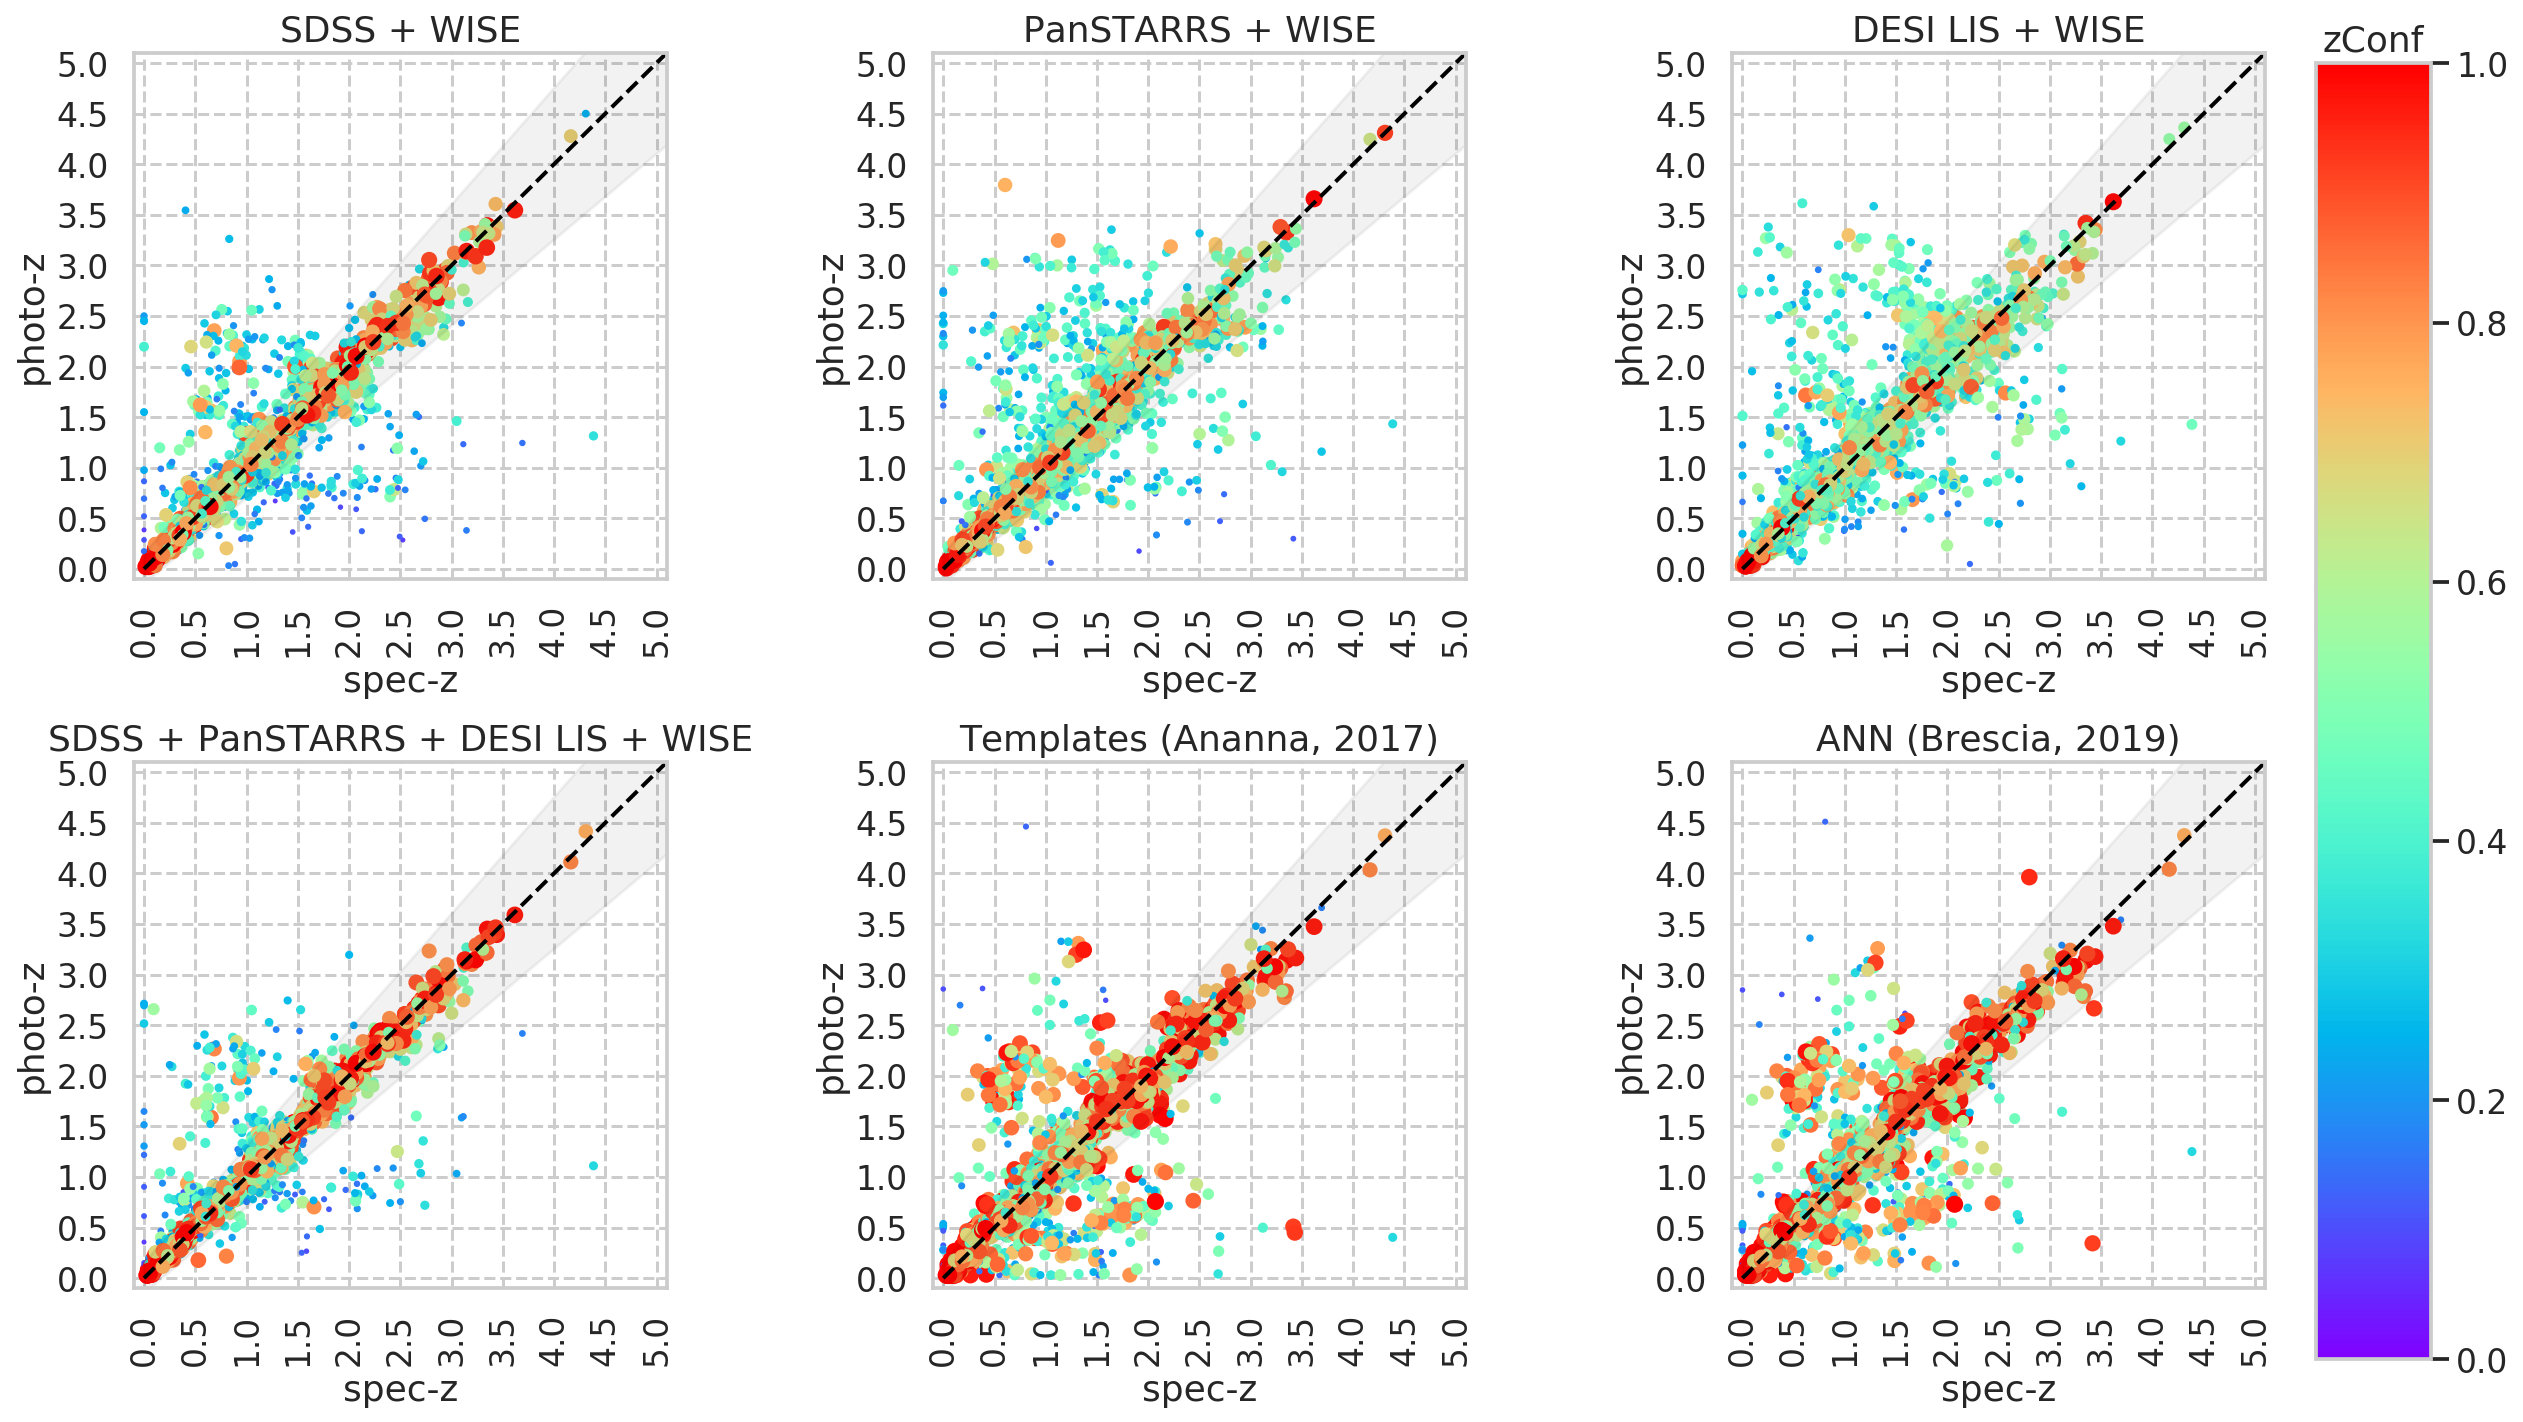
\includegraphics[width=\linewidth]{images/scatterplots-s82x-a17-all30sec.png}
    \caption{Scatterplots on Stripe82X-A17}
    \label{fig:my_label}
\end{figure*}

\begin{figure}
    \centering
    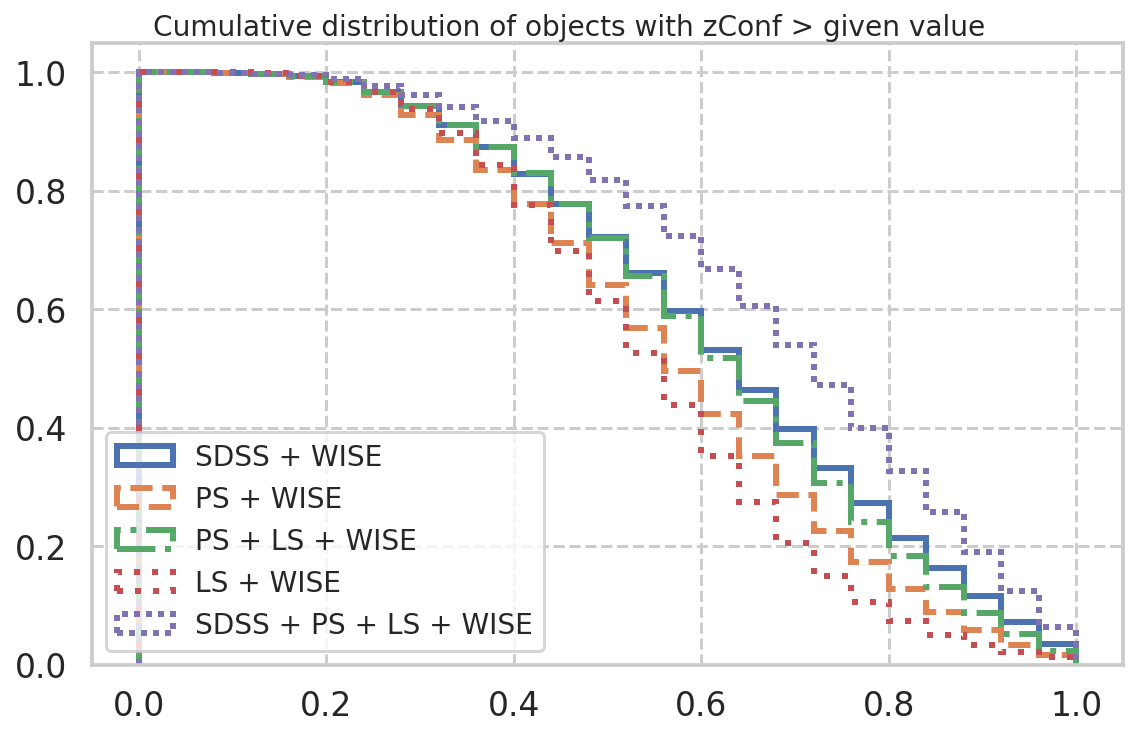
\includegraphics[width=\linewidth]{images/zconfs2-dr16qso.png}
    \caption{zConf cumulative distribution for DR16 qso test}
    \label{fig:zconfs2-dr16qso}
\end{figure}

\subsubsection{Quality of confidence intervals}

То же самое, но по метрикам Колмогорова-Смирнова, квантильный график для доверительных интервалов, сравнение с Ananna и Brescia (они приводят доверительные инттервалы?)

\begin{figure*}
    \centering
    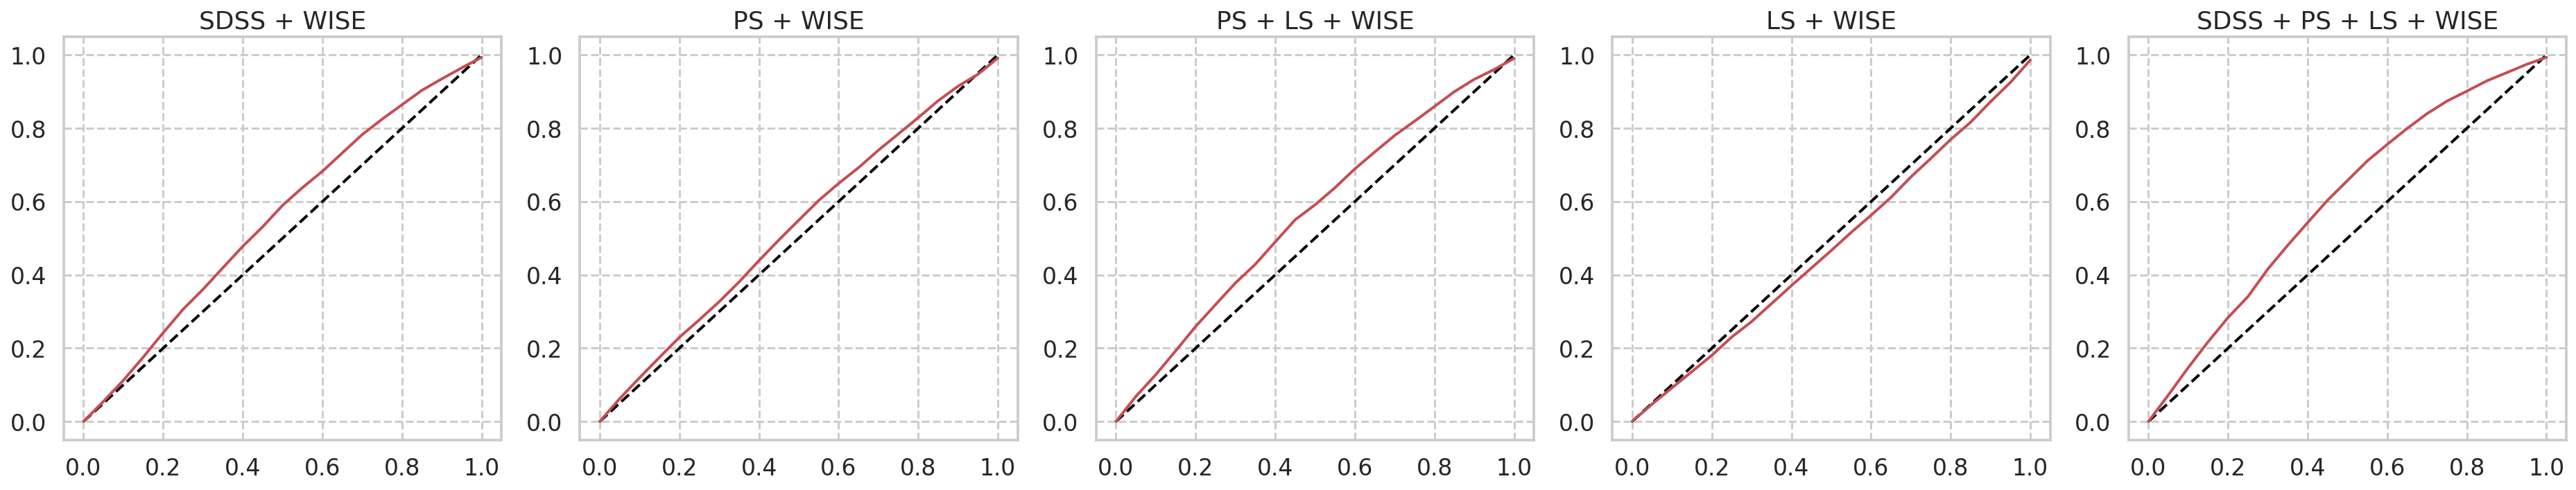
\includegraphics[width=\linewidth]{images/calibration-ci.png}
    \caption{QQ-plot for confidence intervals on Stripe82X test.}
    \label{fig:qqci}
\end{figure*}


\begin{figure*}
    \centering
    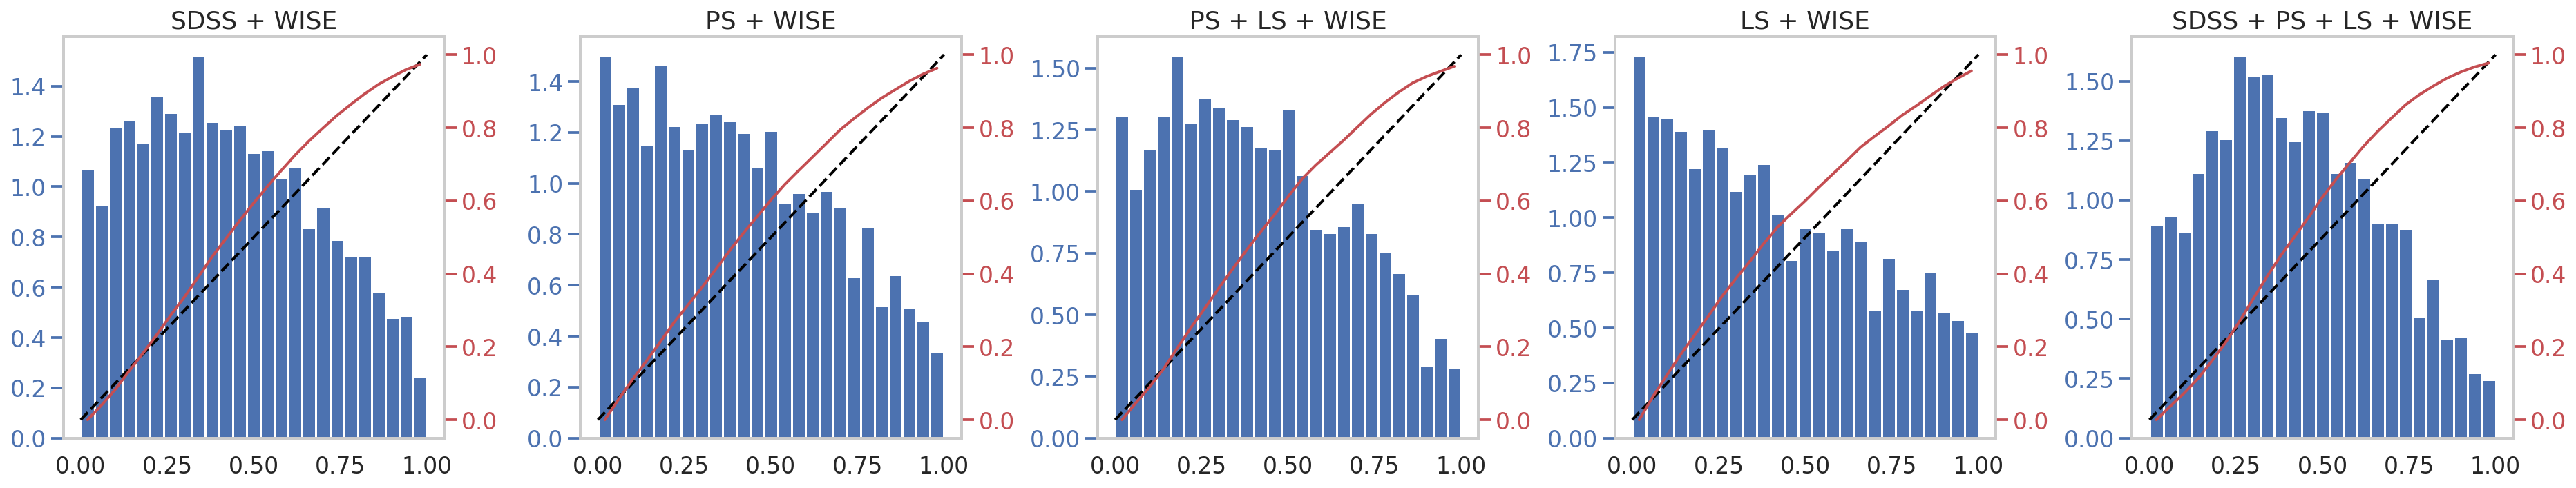
\includegraphics[width=\linewidth]{images/calibration-pit.png}
    \caption{PIT-histogram and QQ-plot for full probabilistic predictions on Stripe82X test.}
    \label{fig:qqpit}
\end{figure*}

Доверительные интервалы немного самоуверенные. Чем точнее модель, тем хуже калибровка.
\section{Conclusions}\label{sec:results}

Проведено исследование, построение и сравнение моделей вероятностных прогнозов фотометрических красных смещений (photo-z) на основе алгоритма случайного леса  с использованием данных современных астрономических обзоров SDSS, PanStarrs и DESI Legacy Survey для построения трехмерной карты квазаров.

Предложена модель photo-z, значительно превосходящая (в ~2 раза) по точности (метрики точечных прогнозов — нормализованное медианное абсолютное отклонение NMAD и доля выбросов n>0.15) лучшие модели (SOTA) известные в литературе. Для рентгеновских источников в тестовой области неба Stripe82X получена точность NMAD = 0.034 / 0.064 / 0.067 и n>0.15 = 0.079 / 0.170 / 0.163 для предложенной модели / шаблонной модели Ananna, 2017 / нейросетевой модели Brescia, 2019, соответственно.

%Предложен алгоритм дополнительной классификации далеких объектов (красное смещение больше 3), превосходящий классификацию по мере достовероности прогноза zConf (предложенный алгоритм: ROC AUC = 0.98; классификация по zConf: ROC AUC = 0.94). При полноте 0.93 достигнуто получено уменьшение доли звезд, ложно классифицированных как квазары (предложенный алгоритм: FPR = 0.10; классификация по zConf: FPR = 0.21).

%Предложен алгоритм постобработки вероятностных прогнозов для улучшения калибровки Temperature Scaling, показана его работоспособность.
\section{Discussion}\label{sec:discussion}

\begin{figure*}
    \centering
    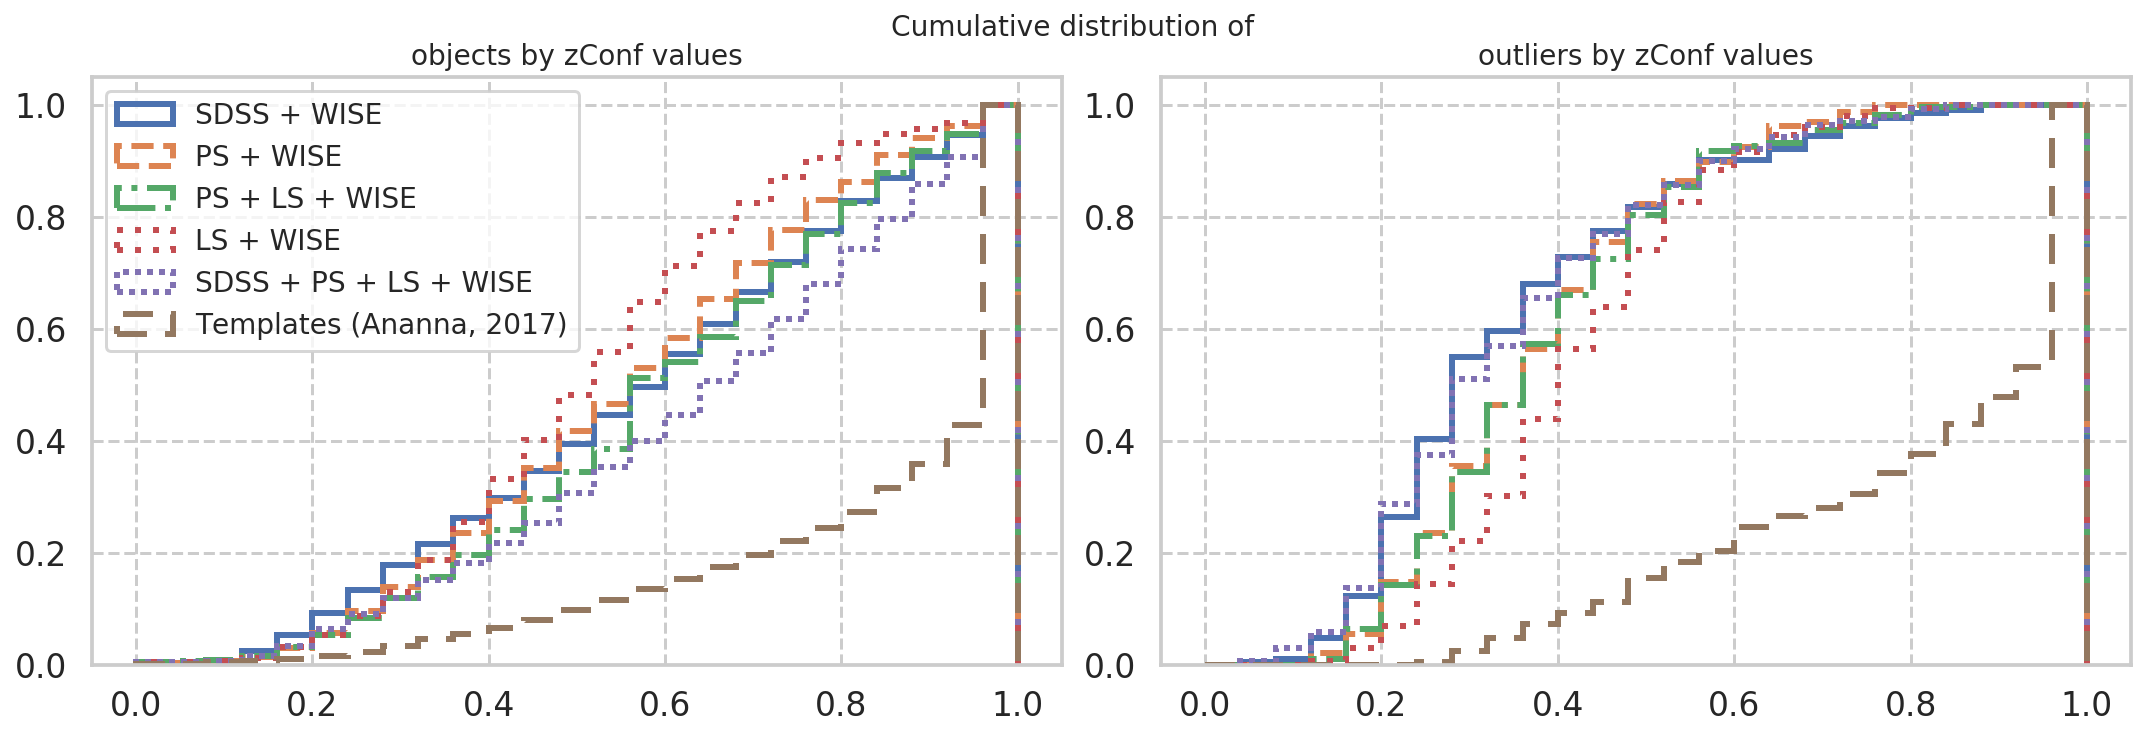
\includegraphics[width=\linewidth]{images/zconfs-s82x-a17.png}
    \caption{zConf cumulative distribution for entire Stripe82X dataset (left) and outliers (right)}
    \label{fig:zconfs-s82x-a17}
\end{figure*}

\begin{figure}
    \centering
    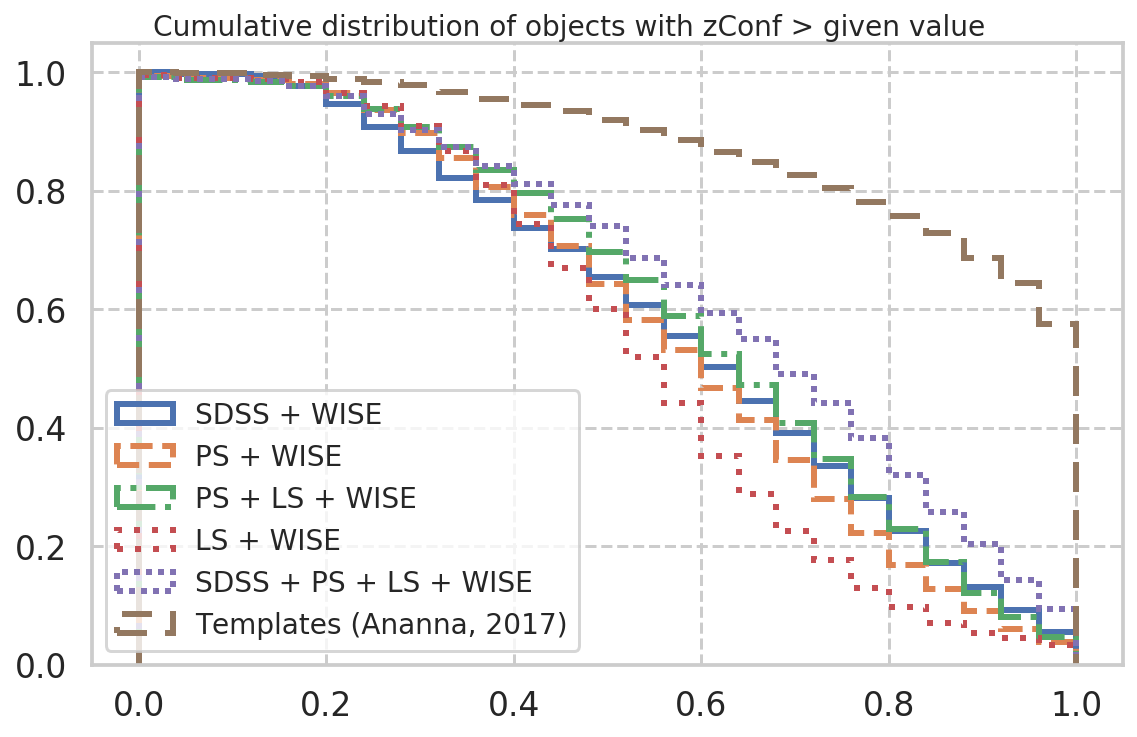
\includegraphics[width=\linewidth]{images/zconfs2-s82x-a17.png}
    \caption{zConf cumulative distribution for Stripe82X dataset}
    \label{fig:zconfs2-s82x-a17}
\end{figure}

Сказать, что результаты Brescia получены на кросс-валидации, у нас - нормальная обучающая выборка.

Обсудить покрытие неба моделями, что хотим хорошую точность на PanStarrs.


\section*{Acknowledgments}
..

% bibliograpgy 
\bibliographystyle{mnras}
\bibliography{main}

\appendix

\section{..}

\end{document}
